\documentclass[review]{elsarticle} %review=doublespace preprint=single 5p=2 column
%%% Begin My package additions %%%%%%%%%%%%%%%%%%%
\usepackage[hyphens]{url}

  \journal{Journal of Archaeological Science: Reports} % Sets Journal name


\usepackage{lineno} % add
\providecommand{\tightlist}{%
  \setlength{\itemsep}{0pt}\setlength{\parskip}{0pt}}

\usepackage{graphicx}
\usepackage{booktabs} % book-quality tables
%%%%%%%%%%%%%%%% end my additions to header

\usepackage[T1]{fontenc}
\usepackage{lmodern}
\usepackage{amssymb,amsmath}
\usepackage{ifxetex,ifluatex}
\usepackage{fixltx2e} % provides \textsubscript
% use upquote if available, for straight quotes in verbatim environments
\IfFileExists{upquote.sty}{\usepackage{upquote}}{}
\ifnum 0\ifxetex 1\fi\ifluatex 1\fi=0 % if pdftex
  \usepackage[utf8]{inputenc}
\else % if luatex or xelatex
  \usepackage{fontspec}
  \ifxetex
    \usepackage{xltxtra,xunicode}
  \fi
  \defaultfontfeatures{Mapping=tex-text,Scale=MatchLowercase}
  \newcommand{\euro}{€}
\fi
% use microtype if available
\IfFileExists{microtype.sty}{\usepackage{microtype}}{}
\bibliographystyle{elsarticle-harv}
\usepackage{longtable}
\usepackage{graphicx}
\ifxetex
  \usepackage[setpagesize=false, % page size defined by xetex
              unicode=false, % unicode breaks when used with xetex
              xetex]{hyperref}
\else
  \usepackage[unicode=true]{hyperref}
\fi
\hypersetup{breaklinks=true,
            bookmarks=true,
            pdfauthor={},
            pdftitle={Stable isotope approach to farming and husbandry practices at Phoenician site of Castro Marim between 8th -- 5th century B.C.E},
            colorlinks=false,
            urlcolor=blue,
            linkcolor=magenta,
            pdfborder={0 0 0}}
\urlstyle{same}  % don't use monospace font for urls

\setcounter{secnumdepth}{5}
% Pandoc toggle for numbering sections (defaults to be off)

% Pandoc citation processing
\newlength{\cslhangindent}
\setlength{\cslhangindent}{1.5em}
\newlength{\csllabelwidth}
\setlength{\csllabelwidth}{3em}
% for Pandoc 2.8 to 2.10.1
\newenvironment{cslreferences}%
  {}%
  {\par}
% For Pandoc 2.11+
\newenvironment{CSLReferences}[2] % #1 hanging-ident, #2 entry spacing
 {% don't indent paragraphs
  \setlength{\parindent}{0pt}
  % turn on hanging indent if param 1 is 1
  \ifodd #1 \everypar{\setlength{\hangindent}{\cslhangindent}}\ignorespaces\fi
  % set entry spacing
  \ifnum #2 > 0
  \setlength{\parskip}{#2\baselineskip}
  \fi
 }%
 {}
\usepackage{calc}
\newcommand{\CSLBlock}[1]{#1\hfill\break}
\newcommand{\CSLLeftMargin}[1]{\parbox[t]{\csllabelwidth}{#1}}
\newcommand{\CSLRightInline}[1]{\parbox[t]{\linewidth - \csllabelwidth}{#1}\break}
\newcommand{\CSLIndent}[1]{\hspace{\cslhangindent}#1}

% Pandoc header
\usepackage{subfig}
\usepackage{booktabs}
\usepackage{longtable}
\usepackage{array}
\usepackage{multirow}
\usepackage{wrapfig}
\usepackage{float}
\usepackage{colortbl}
\usepackage{pdflscape}
\usepackage{tabu}
\usepackage{threeparttable}
\usepackage{threeparttablex}
\usepackage[normalem]{ulem}
\usepackage{makecell}
\usepackage{xcolor}

\usepackage{wasysym}
\usepackage{geometry}
\sloppy

\begin{document}
\begin{frontmatter}

  \title{Stable isotope approach to farming and husbandry practices at Phoenician site of Castro Marim between 8th -- 5th century B.C.E}
    \author[Universidade de Évora,Laboratório HERCULES]{Roshan Paladugu\corref{1}}
   \ead{rpaladugu@uevora.pt} 
    \author[SAPIENZA Università di Roma]{Alessandra Celant}
   \ead{alessandra.celant@uniroma1.it} 
    \author[SAPIENZA Università di Roma]{Federico Di Rita\corref{2}}
   \ead{federico.dirita@uniroma1.it} 
    \author[Universidade de Lisboa]{Ana Margarida Arruda\corref{2}}
   \ead{ana2@campus.ul.pt} 
    \author[Laboratório HERCULES]{Anne-France Maurer\corref{2}}
   \ead{annefrance.maurer@gmail.com} 
    \author[SAPIENZA Università di Roma]{Donatella Magri\corref{2}}
   \ead{donatella.magri@uniroma1.it} 
    \author[Universidade de Évora,Laboratório HERCULES]{Cristina Barrocas Dias\corref{1}}
   \ead{cmbd@uevora.pt} 
      \address[Universidade de Évora]{Departamento de Química, Escola de Ciências e Tecnologia, Universidade de Évora, Colégio Luís António Verney, Rua Romão Ramalho 59, Évora, Portugal (7000-671)}
    \address[Laboratório HERCULES]{Laboratório HERCULES, Universidade de Évora, Palácio do Vimioso, Largo Marquês de Marialva 8, 7000-554 Évora, Portugal}
    \address[SAPIENZA Università di Roma]{Dipartimento di Biologia Ambientale, SAPIENZA Università di Roma, Piazzale A. Moro 5, 00185 Roma, Italy}
    \address[Universidade de Lisboa]{Centro de Arqueologia da Universidade de Lisboa, Faculdade de Letras da Universidade de Lisboa, Alameda da Universidade, 1600-214, Lisboa, Portugal}
      \cortext[1]{Corresponding Author}
    \cortext[2]{Equal contribution}
  
  \begin{abstract}
  This is the abstract.

  It consists of two paragraphs.
  \end{abstract}
  
 \end{frontmatter}

\hypertarget{introduction}{%
\section{Introduction}\label{introduction}}

Iberian Peninsula underwent Oriental colonization by thalassocracy influences originating from the Near East in the Early Iron Age (8th -- early 5th centuries B.C.E). These colonizers, referred to as Phoenicians, were mostly culturally homogeneous and politically independent city-states with the Levant's power nucleus (present-day Lebanon) (Dietler, 2009; Gomes and Arruda, 2018; Quinn, 2019). The city-states served as nodes of an expansive trade network across the Mediterranean, including the Atlantic coast of Europe (Aubet, 2001; Markoe, 2005). It is widely accepted that the main driving force behind this westward expansion was the need to establish a stable supply of metalliferous resources (Arruda, 2009; Aubet, 2001; Eshel et al., 2019; Markoe, 2005). Phoenicians have mined the Iberian Pyrite belt for silver, tin, lead, and copper circa early 800 B.C.E (Eshel et al., 2019; Renzi et al., 2012; Wood et al., 2019). These mined metals were hauled back to the inner Mediterranean region through their well-established networks through posts along the rivers and southern shore of the Iberian Peninsula (Eshel et al., 2019).

The intense and prolonged density of settlements along the Southern Iberian coast cannot simply be explained by the quest for mineral sources, primarily because most of them are situated in locations with neither metallogenic minerals nor indigenous settlements. This settlement pattern is further emphasized by the contrast between the densely clustered settlements of Iberia and sparsely scattered settlements of North Africa. Other factors influencing the settlement density include agricultural resources (Wagner and Alvar, 2003; Wagner and Alvar, 1989), exploitation of marine resources (salt (Manfredi, 1992), and Tyrrhenian Purple production (Uriel, 2000)), timber (Treumann, 2009; Treumann, 1998), and labor force (Arrastio, 2000, 1999). The Phoenician traders had to ensure stable sources of food for the population apart from the industrial activities. Southwestern Iberia has been noted for its rich mineral veins and abundant natural fertility, and the Phoenicians exploited this fertile landscape while actively transforming it -- including cultivable land (Arruda, 2009, 2003; Neville, 1998; Roller, 2014). The Phoenicians' metal exploitation perspective has been studied, but the agricultural aspects have received very little attention. This study aims to shed light on the stable isotope approach to reconstruct the farming strategies and animal husbandry practices in the Phoenician -- Punic period of Portugal, specifically at Castro Marim.

\hypertarget{context}{%
\section{Context}\label{context}}

\hypertarget{phoenician---punic-agriculture}{%
\subsection{Phoenician - Punic Agriculture}\label{phoenician---punic-agriculture}}

Most knowledge about Phoenician and Punic agriculture comes from the famous treaty by Mago, of which only a few fragments have survived and subsequently translated (Martin, 1971). Other accounts are by authors from the Greek and Roman domains, usually written centuries after the demise of the Phoenician -- Punic civilization. The current understanding has been mainly developed due to systematic excavations of different Phoenician -- Punic settlements in Iberia and subsequent zooarchaeological and archaeobotanical studies on the recovered faunal and botanical remains (Aubet, 2001; Wagner and Alvar, 2003; Wagner and Alvar, 1989).
The Southwest Iberian region has been praised by Strabo (3, 2, 8) for possessing the rare combination of abundant mineral deposits and natural fertility (Roller, 2014). From the 9th century B.C.E, Phoenician presence is noted in the Iberian Peninsula along the Atlantic's coastal zone. This strategic location gave them reasonable access to the sailing routes and provided them with a plethora of cultivable land (Aubet, 2001). The colonies in Iberia were located in a landscape similar to that in the Levant with proximity to the coast and marked with steep mountain ranges and riverine valleys. Being located in a river valley gave the colonizers the ease of adapting existing practices from the Mediterranean in the Iberian hinterland. This included modifying and adapting the landscape to suit their agricultural needs, comprising farming and animal husbandry (Gómez Bellard, 2019).

Agricultural techniques from the East, such as irrigation, were used to improve upon the native practices. The iron production technology gave more robust implements such as plowshare etc., to the farmers. Better yielding cultivars (Eg: grapes and olives) and new species of animals (Eg: horse, donkey, and chicken) were introduced (Davis, 2007; Queiroz et al., 2006). Following the ``sixth century crisis,'' the colonies in Iberia came under Carthage's influence, and this period is referred to as the Punic period (Arruda et al., 2013). The crisis had multiple facets of which one of the leading cause was the exhaustion of Iberia's mineral resources. This crisis forced the settlements to change their economy from an industry-driven one to a more agronomic-based one. This economic change brought a drastic change in space use concerning both settlement and domain. In the Punic period, in addition to the cultivation of cash crops and wine, local usable arboreal products were identified and exploited to boost exports (Gómez Bellard, 2019; Neville, 1998). The exploitation of arboreal products and perennial crops meant the existence of both short-term and long-term agricultural investments. Such diverse investments with different harvest times must have led to the development of a complex agricultural economy.

\begin{figure*}
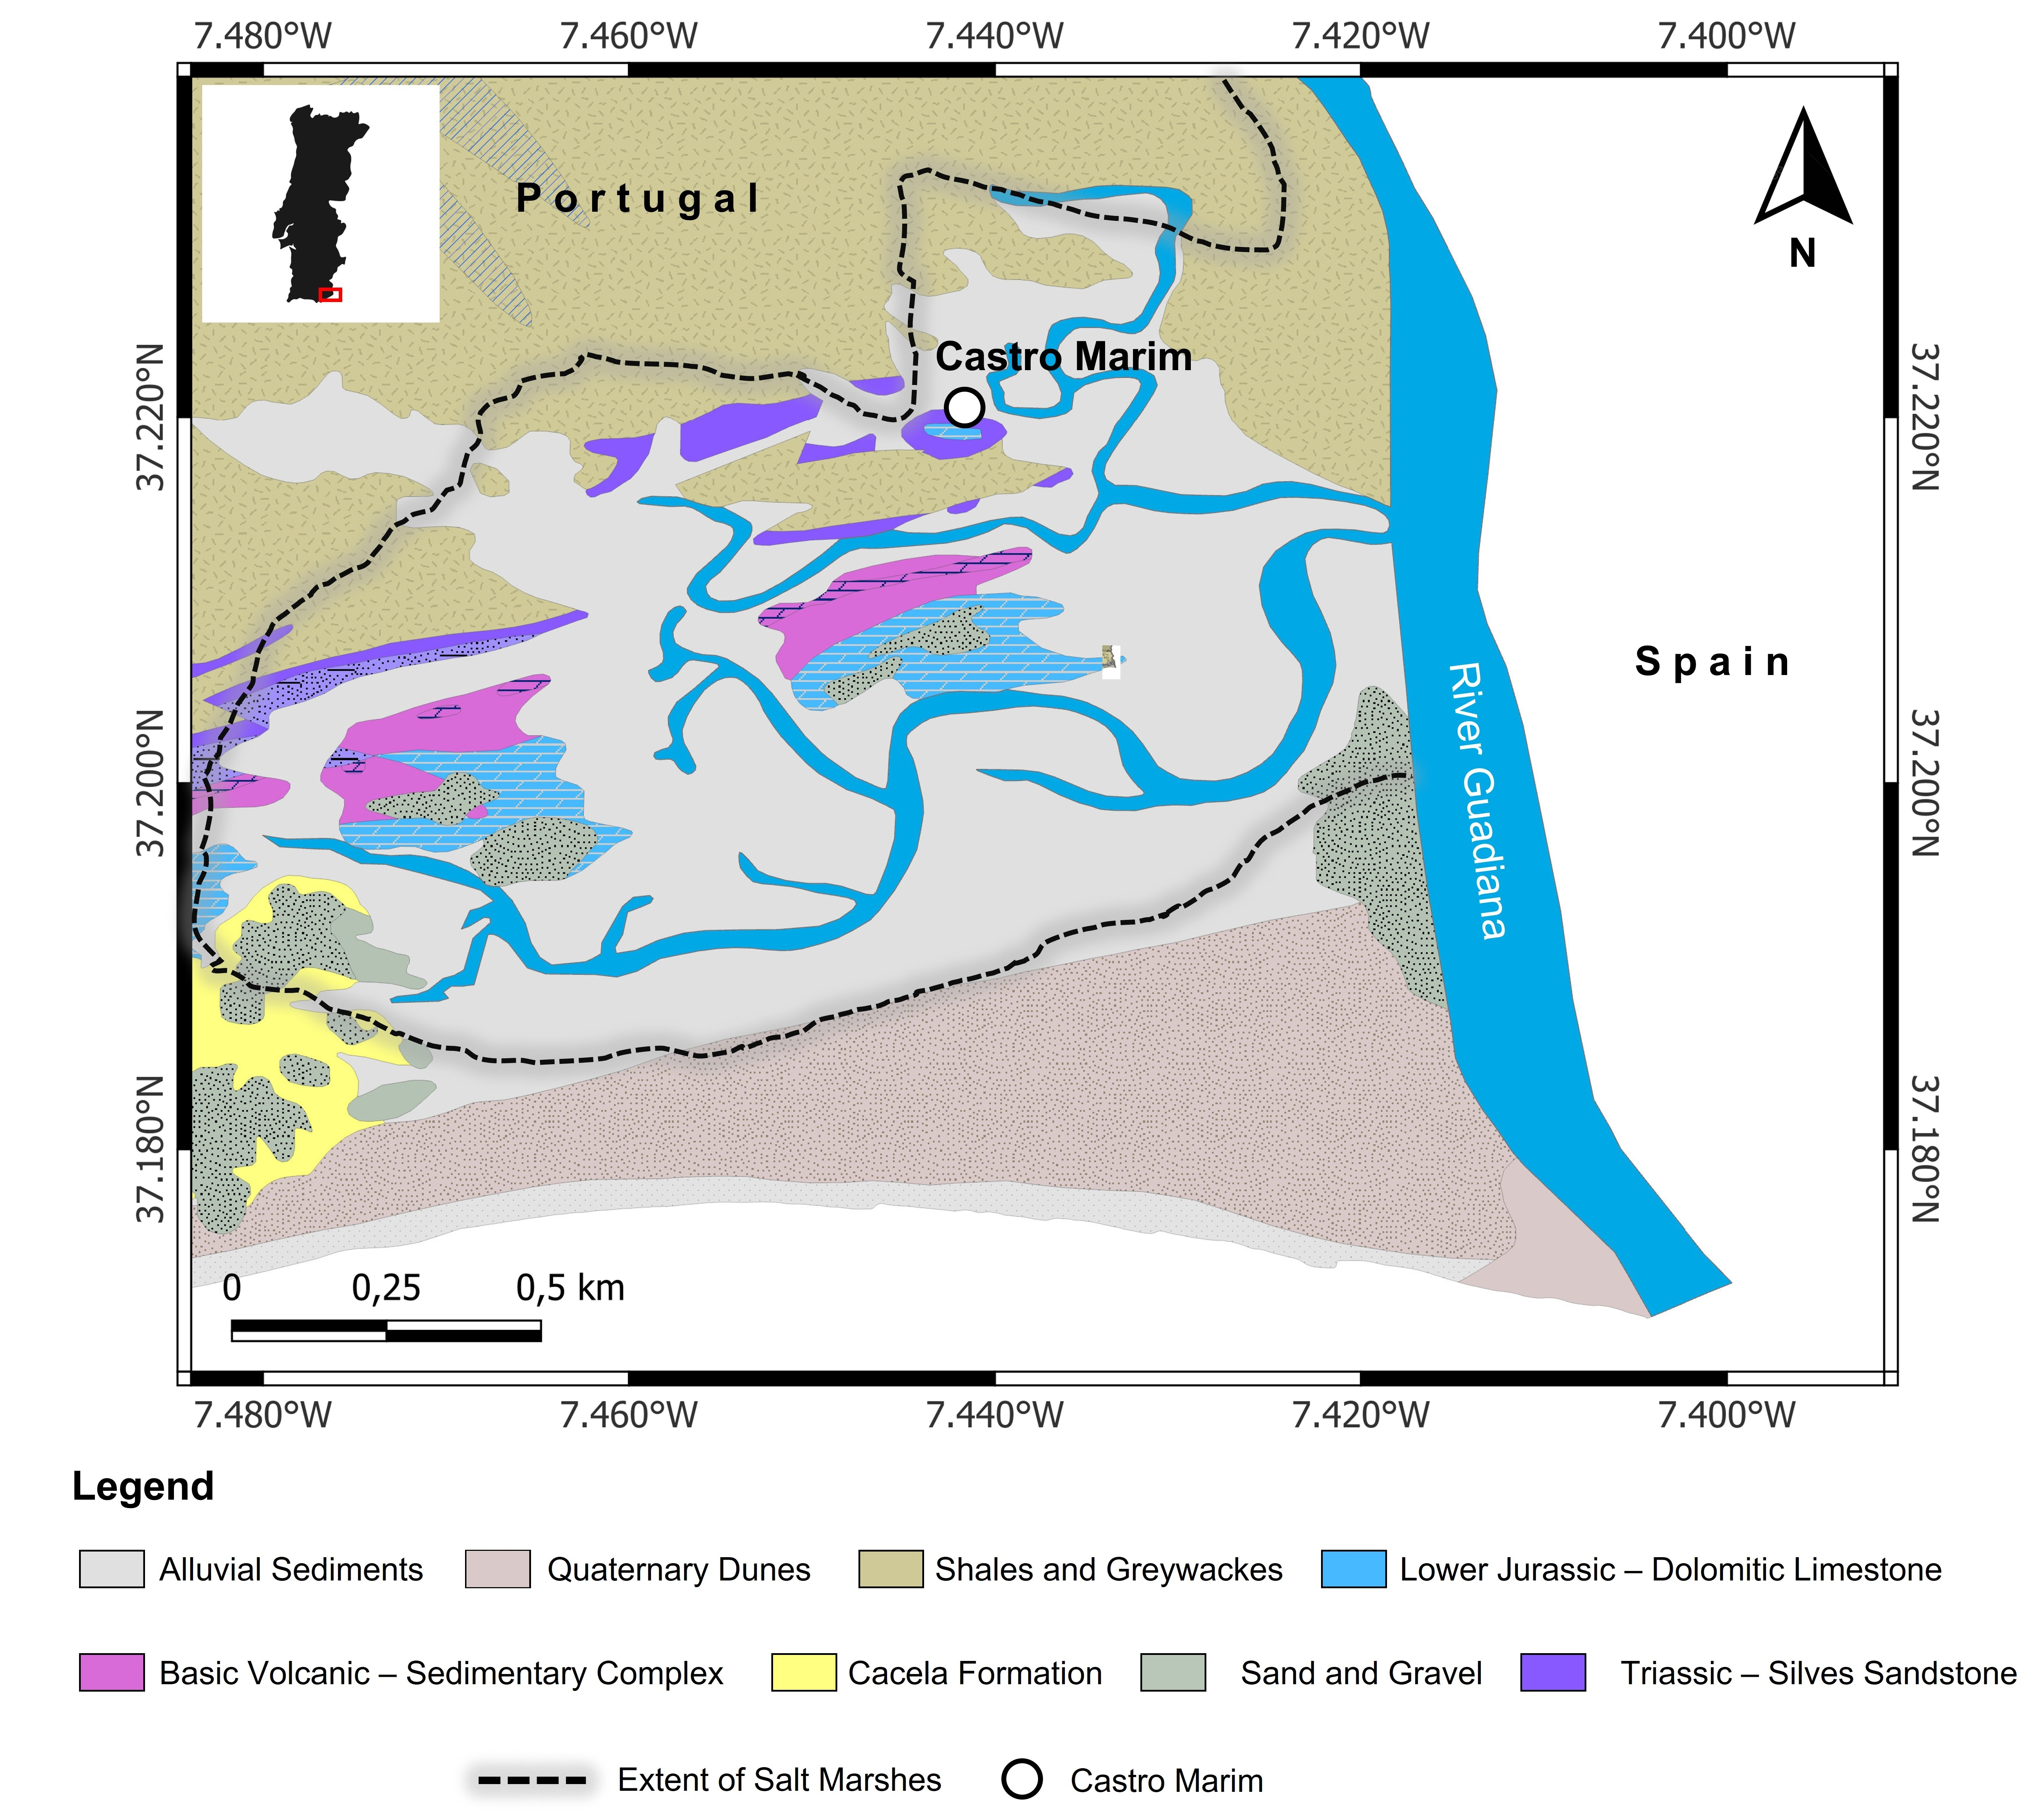
\includegraphics[width=0.98\textwidth]{C:/Users/rosha/Documents/R/Projects/castro_marim_phoenician/./images/castro_marim_map} \caption{Map indicating the location of Castro Marim on the banks of Guadiana Estuary, Algarve Region of Portugal (www.openstreetmap.org).}\label{fig:castro-marim-loc}
\end{figure*}

\hypertarget{site-background}{%
\subsection{Site Background}\label{site-background}}

Castro Marim is located on the Guadiana estuary (Fig. \ref{fig:castro-marim-loc}) as a portal to the metallogenic mineral-rich Baixo -- Alentejo region as well as to the fertile cultivable lands in the interior regions. The Iron Age settlement was located on an elevation with adequate natural defensive elements and overlooked vast swatches of land, which allowed domination of estuarine traffic and agricultural activities in its domain of influence. These conditions allowed trade and cultural networks between the indigenous communities with the Mediterranean communities to flourish. The earliest human activities are traced back to the Late Bronze Age with East-West orthogonal settlement architecture around the first half of 7th century B.C.E, in the Orientalising period (Arruda et al., 2013; Arruda, 1996). Phoenician imports and other human presence signs declined from the second half of 6th-century B.C.E till the first half of 5th-century B.C.E (Arruda, 1996). Significant changes in material culture and restructuring of the settlement architecture with a Northeast -- Southwest orientation are observed from the second half of the 5th-century B.C.E (Arruda et al., 2013, 2006; Arruda and Freitas, 2008). The earlier period's departure was marked with imports from Greek products -- specifically ceramics such as kilikes, skyphoi, and kantharoi (Arruda et al., 2013). This resurgence put Castro Marim back in the Phoenician string of pearls along the Iberian Peninsula's Atlantic coast till the 3rd-century B.C.E (Arruda et al., 2013, 2006; Neville, 1998; Niemeyer, 1984). The Phoenician -- Punic period is represented by archaeological phases III, IV, and V.

Being in a littoral zone made it was possible to adopt a wide range of agricultural strategies and husbandry practices at Castro Marim. The presence of cereals (\emph{Hordeum} / \emph{Triticum}), grapes (\emph{Vitis}), pulses (\emph{Vicia} / \emph{Cicer}), and other cultivated species (\emph{Olea} / \emph{Coriandrum}) as well as exploitation of wild woody plants (\emph{Pinus} / \emph{Arbutus} etc.) have been elucidated from the archaeological record (Queiroz et al., 2006). The animals (native to Portugal) include cattle (\emph{Bos taurus}), goat (\emph{Capra hircus}), sheep (\emph{Ovis aries}), pig (\emph{Sus scrofa/domesticus}), red deer (\emph{Cervus elaphus}), and rabbit (\emph{Oryctolagus cuniculus}) (Davis, 2007). The sudden arrival of chicken (\emph{Gallus domesticus}) has been documented, which the Phoenicians introduced in the second half of 5th-century B.C.E (Davis, 2007).

\hypertarget{zooarchaeological-assessment}{%
\subsection{Zooarchaeological assessment}\label{zooarchaeological-assessment}}

Davis, 2007 carried out the zooarchaeological assessment. Ovicaprids (sheep and goats) followed by pigs and cattle dominate the Castro Marim mammal taxa. Both sheep and goats were equally represented with negligible fluctuations throughout the Iron Age at Castro Marim. The wild species in the assemblage consisted mainly of red deer and rabbits. It is worth mentioning here that no morphometric distinction could be made between wild and domesticated pigs. Both the species are present consistently in all the phases of the settlement. It is worth mentioning that the wild relative of the domesticated pig was not distinguishable from the latter. There is a spike in the presence of bird remains in the later phases of the Iron Age (Phase IV - V), primarily due to the introduction of domesticated chicken. The presence of partridge, a common wild species of Iberia, is also noted. Unlike the chicken, partridge has never been domesticated. Ovicaprids and cattle were kept well into maturity as they were prized more for their secondary purposes than their meat. Sheep and goat were kept for their milk and wool, usually slaughtered after they reach at least two years of age. Cattle were valued for their power to plow in the fields as well as to pull heavy loads. Also, they too were a source of milk. Pigs, on the other hand, were slaughtered as juveniles as they were primarily reared for slaughter. Most of the red deer found were adults, suggesting a hunting preference of that period as a vital subsidiary source of meat. Chicken seems to be slaughtered at a young age, whereas the partridges at an adult age. The slaughter age indicates the domesticated status of chicken and wild status of partridge, respectively.

\hypertarget{archaeobotanical-assessment}{%
\subsection{Archaeobotanical assessment}\label{archaeobotanical-assessment}}

The original archaeobotanical assessment was carried out by Queiroz et al. (2006). Cereals make up the most significant fraction of the carpological remains. The bulk of cereals is barley (\emph{Hordeum vulgare}) with a tiny fraction of wheat (\emph{Triticum durum/aestivum}). Pulses are mainly broad beans (\emph{Vicia faba}) and chickpeas (\emph{Cicer arietinum}), of which the former has been present in Portugal since prehistoric times, whereas the latter is introduced as a luxury food in the Roman period from Asia. The presence of grape (\emph{Vitis vinifera/sylvestris}) seeds and carbonized wood is typical, starting from the Roman period in Portugal. The presence of grape seeds in Iron Age Castro Marim indicates cultivation by the local population. The most exciting carpological remains are of coriander (\emph{Coriandrum sativum}) which is not native to Portugal and was supposed to be introduced during medieval times, making this the earliest coriander occurrence in Portugal. Charred pine, oak, ash, and poplar wood were recovered abundantly. The exploitation of wild woody plants for timber and fruits marks the Iberian peninsula's Phoenician colonization. Due to unforeseen circumstances, these identified remains could not be accessed for isotope analyses. Previously unprocessed sediments were studied again to gain botanical remains.

\hypertarget{methodological-approach}{%
\section{Methodological approach}\label{methodological-approach}}

\hypertarget{zooms-analysis-of-ovicaprids}{%
\subsection{ZooMS Analysis of Ovicaprids}\label{zooms-analysis-of-ovicaprids}}

Skeletal elements of goats and sheep are a common occurrence in archaeological contexts. A major issue plaguing comparative husbandry studies between sheep and goat is the overlap of skeletal elements (Boessneck et al., 1964; Payne, 1969; Schramm, 1967). This is further complicated by the environmental modifications which erode diagnostic markers and produce undistinguishable fragments (Buckley et al., 2010). Zooarchaeology by Mass Spectrometry (ZooMS) is a high-throughput analytical technique which can discriminate unidentifiable bone fragments. ZooMS exploits the the genetically distinct alpha 2 (\(\alpha2\)) chain of the collagen (I) protein to distinguish between different species. Collagen is the most abundant protein in mammalian tissues and this allows for its extraction in most scenarios where DNA cannot be retrieved (Lyman, 1994). The genus \emph{Capra} is identified by an m/z at 3093 whereas that of \emph{Ovis} has a peptide marker with an observed m/z at 3033 (Buckley et al., 2010).

\hypertarget{stable-isotope-analysis-of-plants-and-animals}{%
\subsection{Stable isotope analysis of plants and animals}\label{stable-isotope-analysis-of-plants-and-animals}}

Stable isotope (\(\delta ^{13}C\), and \(\delta ^{15}N\)) analyses of faunal bones are valuable means of reconstructing foddering practices and other animal husbandry aspects (Price et al., 2017). The variation in \(\delta ^{13}C\) of terrestrial organisms is determined by the primary producers' photosynthetic pathway, distinguished as C\textsubscript{3}, C\textsubscript{4}, and CAM plants (DeNiro and Epstein, 1978; Farquhar et al., 1989; Kohn, 2010; Tieszen, 1991). Plant species are overwhelmingly C\textsubscript{3} in nature, including most cultivated plants such as barley, wheat, oats, potato, and other wild edible plants (Fernández-Crespo et al., 2019). C\textsubscript{4} plants consist primarily of tropical grasses, millets, sugarcane, corn, and sorghum. C\textsubscript{4} plants thrive in warm and high-temperature environments and thus are restricted to coastal zones in regions with temperate climates (Leegood, 2013; Price et al., 2017). \(\delta ^{13}C\) measurements are also helpful to differentiate between terrestrial and aquatic food sources (Froehle et al., 2010; Kellner and Schoeninger, 2007). \(\delta ^{15}N\) values indicate the isotopic composition of the consumers and their dietary intake to consumers in a food chain (Price et al., 2017). \(\delta ^{15}N\) values can also be used to distinguish between terrestrial and marine diets (Deniro and Epstein, 1981; Webb et al., 2017), consumption of manured, and unmanured crops (Bogaard et al., 2013; Deniro and Epstein, 1981; Fernández-Crespo et al., 2019; Fraser et al., 2013), and trophic level within an established ecosystem (Hedges and Reynard, 2007; Schoeninger, 1985).

There are only two significant inputs, which humans can manipulate to cultivate plants: water and nitrogen input. Variation in \(\delta ^{13}C\) values of plants is primarily due to water availability as any dry spells affect the movement of carbon dioxide through the stomata (Ferrio et al., 2007; Ferrio et al., 2005). The water status of crops can be artificially controlled by irrigation regimes which are also reflected in \(\delta ^{13}C\) values (Ferrio et al., 2005; Wallace et al., 2013). It is essential to convert the absolute \(\delta ^{13}C\) values to carbon discrimination values to facilitate the comparison with the values of the modern crops grown under controlled watering regimes (Farquhar et al., 1989; Wallace et al., 2013):

\[\Delta^{13}C = \frac{\delta ^{13}C_{air} - \delta ^{13}C_{plant}}{1+\delta ^{13}C_{plant}/1000}\]
Another major factor, which affects the \(\delta ^{13}C\) measurements, is the canopy effect where forested areas are more depleted in the heavier \textsuperscript{13}C isotope compared to open areas (Bonafini et al., 2013). One of the most ancient practices to increase soil fertility is by manuring with animal waste as animal manure is much higher than endogenous soil in terms of nitrogen isotopic composition (Bogaard et al., 2013). Usually, the plants treated with manure exhibit higher \(\delta ^{15}N\) values (as much as 10\permil) when compared to unfertilized plants (Bogaard et al., 2007; Fraser et al., 2011). The \(\delta ^{13}C\) and \(\delta ^{15}N\) values themselves do not reveal the agricultural practices but reveal patterns when interpreted within the context of a specific site.

The mean \(\delta ^{34}S\) value of terrestrial sources is assumed to be 0\permil. Inorganic sulfur enters the food web through plants from the weathered bedrock (in a complete terrestrial setting), precipitation (sea spray), and microbial activity due to flooding events (Nitsch et al., 2019). As the inorganic sulfur passes through the food web in the form of proteins, only a negligible fractionation occurs between diet and consumer (Hobson, 1999; Nehlich, 2015). Thus, the \(\delta ^{34}S\) ratio of collagen closely reflects that of the native water source, bedrock, and soluble sulphur-bearing minerals.

\begingroup\fontsize{7.5}{9.5}\selectfont

\begin{longtable}[t]{ccccc}
\caption{\label{tab:table1}Collagen yield and FT-IR results (IRSF and C/P) of selected faunal bone samples.}\\
\toprule
Sample ID & Phase & Collagen yield (\%) & IRSF & C/P\\
\midrule
\endfirsthead
\caption[]{\label{tab:table1}Collagen yield and FT-IR results (IRSF and C/P) of selected faunal bone samples. \textit{(continued)}}\\
\toprule
Sample ID & Phase & Collagen yield (\%) & IRSF & C/P\\
\midrule
\endhead

\endfoot
\bottomrule
\endlastfoot
CMOF435 & III & 10.9 & 2.98 & 0.21\\
CMOF397 & III & 13.3 & 2.87 & 0.43\\
CMOF388 & III & 6.7 & 2.59 & 0.29\\
CMOF424 & III & 45.7 & 2.48 & 0.21\\
CMOF230 & III & 8.4 & 3.01 & 0.37\\
CMOF181 & III & 24.6 & 2.97 & 0.26\\
CMOF158 & III & 5.1 & 2.78 & 0.40\\
CMOF779 & III & 2.5 & 2.43 & 0.26\\
CMOF370 & III & 41.6 & 2.78 & 0.38\\
CMOF373 & III & 6.3 & 2.60 & 0.39\\
CMOF402 & III & 12.3 & 2.45 & 0.36\\
CMOF374 & III & 15.6 & 2.41 & 0.41\\
CMOF254 & IV & 7.2 & 3.01 & 0.32\\
CMOF756 & IV & 8.8 & 2.53 & 0.33\\
CMOF419 & IV & 9.6 & 3.14 & 0.41\\
CMOF439 & IV & 6.6 & 3.24 & 0.25\\
CMOF677 & IV & 6.2 & 2.51 & 0.34\\
CMOF201 & IV & 29.1 & 2.96 & 0.37\\
CMOF420 & IV & 19.8 & 2.66 & 0.21\\
CMOF463 & IV & 5.3 & 2.93 & 0.20\\
CMOF480 & IV & 10.8 & 2.56 & 0.40\\
CMOF673 & IV & 20.9 & 2.40 & 0.37\\
CMOF660 & IV & 4.0 & 2.60 & 0.28\\
CMOF656 & IV & 49.1 & 2.50 & 0.38\\
CMOF260 & IV & 6.8 & 2.61 & 0.34\\
CMOF147 & IV & 19.8 & 2.62 & 0.40\\
CMOF354 & IV & 41.4 & 2.75 & 0.28\\
CMOF253 & IV & 16.2 & 2.65 & 0.37\\
CMOF467 & V & 15.5 & 2.64 & 0.36\\
CMOF338 & V & 6.0 & 2.61 & 0.22\\
CMOF99 & V & 6.5 & 3.12 & 0.20\\
CMOF466 & V & 19.8 & 2.59 & 0.23\\
CMOF710 & V & 4.5 & 2.63 & 0.25\\
CMOF'737 & V & 6.3 & 2.79 & 0.23\\
CMOF774 & V & 10.5 & 2.87 & 0.35\\
CMOF750 & V & 6.0 & 2.65 & 0.41\\
CMOF323 & V & 2.6 & 3.33 & 0.29\\
CMOF508 & V & 3.0 & 2.50 & 0.23\\
CMOF751 & V & 31.1 & 3.28 & 0.31\\
CMOF772 & V & 3.1 & 2.91 & 0.22\\
CMOF743 & V & 4.5 & 2.74 & 0.22\\
CMOF14 & V & 7.9 & 2.59 & 0.34\\
CMOF777 & V & 3.9 & 3.37 & 0.40\\
CMOF691 & V & 6.8 & 2.79 & 0.42\\
CMOF457 & V & 4.9 & 2.81 & 0.23\\
CMOF468 & V & 22.9 & 3.27 & 0.30\\
CMOF746 & V & 24.7 & 2.54 & 0.28\\
CMOF744 & V & 6.5 & 2.37 & 0.41\\
CMOF731 & V & 10.4 & 2.54 & 0.30\\
CMOF730 & V & 15.8 & 2.48 & 0.30\\
CMOF709 & V & 29.1 & 3.12 & 0.40\\
CMOF643 & V & 8.4 & 2.69 & 0.28\\
CMOF504 & V & 10.9 & 2.69 & 0.36\\
CMOF477 & V & 10.8 & 2.59 & 0.22\\
CMOF394 & V & 21.4 & 2.47 & 0.24\\
CMOF393 & V & 36.2 & 2.39 & 0.42\\
CMOF353 & V & 23.1 & 3.31 & 0.20\\
CMOF334 & V & 11.0 & 3.26 & 0.31\\
CMOF324 & V & 7.7 & 2.79 & 0.42\\
CMOF303 & V & 17.8 & 2.39 & 0.28\\
CMOF94 & V & 34.0 & 3.14 & 0.37\\
CMOF745 & V & 4.5 & 2.83 & 0.30\\*
\end{longtable}
\endgroup{}

\hypertarget{materials-and-methods}{%
\section{Materials and Methods}\label{materials-and-methods}}

\hypertarget{sample-selection}{%
\subsection{Sample Selection}\label{sample-selection}}

Fifty faunal bone samples (Table \ref{tab:table4}) from conclusively adult individuals as well as 9 charred plant macro-remains of \emph{Hordeum vulgare} subsp. \emph{vulgare}, \emph{Hordeum vulgare} subsp. \emph{nudum}, and \emph{Pinus} sp. each have been selected for this study. The sampled faunal bones represent the Phoenician -- Punic period of the settlement (phases III, IV, and V), whereas the charred plant macro -- remains are from only from phase V due to the absence of plant remains from the older phases.

\hypertarget{archaeobotanical-analysis}{%
\subsection{Archaeobotanical Analysis}\label{archaeobotanical-analysis}}

\begin{table}[!h]

\caption{\label{tab:table2}Recovered botanical remains from archaeological sediments.}
\centering
\fontsize{7.5}{9.5}\selectfont
\begin{tabular}[t]{>{}lcc}
\toprule
Species & Recovered Quantity & Phase\\
\midrule
\em{Hordeum vulgare (vulgare/nudum)} & 1300 & V\\
\em{Triticum aestivum/durum} & 4 & V\\
\em{Apium sp.} & 1 & V\\
\em{Pinus sp.} & 2 & V\\
\em{Brassica nigra} & 3 & V\\
\em{Pisum sativum} & 1 & V\\
\em{Galeopsis tetrahit} & 1 & V\\
\em{Vicia faba} & 2 & V\\
\bottomrule
\end{tabular}
\end{table}

200 grams of sediment from each stratigraphic layer of the excavation site was weighed and handpicked for plant macro remains (fruits and charcoal). The recovered remains were examined under a stereo-microscope and taxonomically identified (Table \ref{tab:table2}).

\hypertarget{bone-preservation-fourier-transform-infrared-spectroscopy}{%
\subsection{Bone Preservation: Fourier Transform Infrared Spectroscopy}\label{bone-preservation-fourier-transform-infrared-spectroscopy}}

500 -- 700 mg of bone was cut using a DREMEL\(\text{\textregistered}\) rotary drill with a diamond disc and cleaned of dirt, discoloration, and other foreign content with a dental burr. In addition, compact bone was sampled over spongy bone. Bone fragments were slightly polished with fine sandpaper to obtain a flat surface (Hollund et al., 2013). Infrared spectra were collected using a Bruker\(^\text{\textregistered}\) Alpha\(^\text{\texttrademark}\) Spectrometer with a single-reflection diamond crystal ATR module. Each spectrum was obtained by an accumulation of 128 scans with a spectral resolution of 4 cm\textsuperscript{-1}, from 2000 cm\textsuperscript{-1} to 375 cm\textsuperscript{-1}. Infrared Splitting Factor (IRSF) and relative carbonate content (C/P) were calculated using absorbance heights at 565 cm\textsuperscript{-1}, 590 cm\textsuperscript{-1}, 605 cm\textsuperscript{-1}, 1035 cm\textsuperscript{-1}, and 1415 cm\textsuperscript{-1} wavenumbers (Trueman et al., 2008; Weiner and Bar-Yosef, 1990; Wright and Schwarcz, 1996).

\hypertarget{pretreament-of-macrobotanical-remains}{%
\subsection{Pretreament of macrobotanical remains}\label{pretreament-of-macrobotanical-remains}}

In carbonized plant macro remains, barley grain samples consist of at least 10 whole grains, and pine samples consist of 1 fruit. Morphologically intact samples were chosen after examination under a stereomicroscope (7-45x magnification) and removing any visibly adhering foreign contaminant. An acid-base-acid (ABA) treatment was applied as a pre-treatment (Bogaard et al., 2013; Fraser et al., 2013). First, the samples are treated with 10 mL of 0.5 M HCl at 70 \(\text{\textdegree}\)C for 60 minutes (or until effervescing stops) and then rinsed with ultrapure water until a neutral pH was achieved. 10 mL of 0.1 NaOH solution was added to the samples at 70 \(\text{\textdegree}\)C for 60 minutes and then rinsed with ultrapure water to achieve a neutral pH. Finally, the samples were treated with 0.5 M HCl at 70 \(\text{\textdegree}\)C for 30-60 minutes, followed by 3 rinses with ultrapure water and subsequent freeze-drying.

\hypertarget{collagen-extraction}{%
\subsection{Collagen Extraction}\label{collagen-extraction}}

The modified Longin (1971) method was used to extract collagen from faunal bones (Richards and Hedges, 1999). Approximately 600 mg of bone sample was demineralized using 0.5 M HCl at 4 \(\text{\textdegree}\)C for a fortnight with daily vortex and an acid change after 7 days. Repeated rinses with ultrapure water to reach neutral pH were performed, and the demineralized bones were subjected to an overnight treatment in 0.125 M NaOH at room temperature to remove fulvic and humic acid contamination. The samples were then rinsed repeatedly with ultrapure water to achieve neutrality and gelatinized in 0.01 M HCl at 70 \(\text{\textdegree}\)C for 48 hours. The impurities were separated by filtering the collagen-containing liquid fraction using Ezee -- Filter\(^\text{\texttrademark}\) filters (Elkay\(^\text{\textregistered}\) Laboratory Products). The solubilized collagen was frozen and subsequently lyophilized for 48 hours.

\hypertarget{stable-carbon-and-nitrogen-isotope-analysis}{%
\subsection{Stable carbon and nitrogen isotope analysis}\label{stable-carbon-and-nitrogen-isotope-analysis}}

0.5 - 0.7 mg of freeze-dried collagen powder/barley grain samples were weighed in tin capsules and combusted in an elemental analyzer (EA) with oxygen (Flash 2000 HT\(^\text{\texttrademark}\), Thermo Fisher Scientific\(^\text{\textregistered}\), Bremen, Germany) using pure helium as carrier gas. Isotopic ratios were obtained on a Delta V Advantage Continuous Flow\(^\text{\texttrademark}\) -- Isotope Ratio Mass Spectrometer (Thermo Fisher Scientific\(^\text{\textregistered}\), Bremen, Germany). The raw machine output was normalised by a three-point calibration using international standard reference materials (SRM), namely IAEA-CH-6 (sucrose, \(\delta ^{13}C\) = -- 10.499\permil), IAEA-600 (caffeine, \(\delta ^{13}C\) = -- 27.771\permil; \(\delta ^{15}N\) = + 1\permil), and IAEA-N-2 (ammonium sulphate, \(\delta ^{15}N\) = + 20.3\permil) and in-house standard L-Alanine (\(\delta ^{13}C\) = -- 19.17\permil; \(\delta ^{15}N\) = + 4.26\permil). The standards are regularly (after eleven analyses) included in the analytical routine to correct for instrumental drifts. The isotope values are expressed in per mille (\permil) relative to VPDB (Vienna Pee-Dee Belemnite) for carbon and AIR (Ambient Inhalable Reservoir) for nitrogen. In order to correct for charring effect in plant remains, 0.11\permil and 0.31\permil were subtracted from their \(\delta ^{13}C\) and \(\delta ^{15}N\) values respectively (Nitsch et al., 2015). The fluctuations in \(\delta ^{13}C\) of the atmospheric CO\textsubscript{2} throughout the Holocene were considered while interpreting the stable carbon isotope ratios. The \(\delta ^{13}C\) of atmospheric CO\textsubscript{2} during the period in the study was approximated using the AIRCO\textsubscript{2}\_LOESS system, and then this value was used to compute the \(\delta ^{13}C\) discrimination of plants independent of the source CO\textsubscript{2} (Farquhar et al., 1982; Ferrio et al., 2005).

\hypertarget{stable-sulphur-isotope-analysis}{%
\subsection{Stable sulphur isotope analysis}\label{stable-sulphur-isotope-analysis}}

The collagen samples were combusted with additional V\textsubscript{2}O\textsubscript{5} and a oxygen pulse (IsoPrime\(^\text{\texttrademark}\) Mass spectrometer, Elementar Analysensysteme GmbH\(^\text{\textregistered}\), Langenselbold, Germany). Calibration of \(\delta ^{34}S\) values was performed using international inorganic standards for stable sulphur isotope analysis: NBS127 (+20.3\permil) and IAEA S1 (-0.3\permil). B2155 protein (+6.96 ± 0.04\permil) was used as an internal quality control standard. Stable sulphur isotope values are reported in parts per thousand relative to Vienna-Canyon Diablo Troilite (VCDT).

\hypertarget{statistical-analysis}{%
\subsection{Statistical Analysis}\label{statistical-analysis}}

The obtained data were subjected to statistical analysis using R programming language (R Core Team, 2020; Wickham, 2016). Initially, means and standard deviations were calculated per species. Z-scores were calculated to detect the presence of outliers. Deviance from normal distribution was assessed using Shapiro-Wilks test. F-tests were first used to check for significant equal variance, and subsequently, unpaired Student's t-tests were used for two-sample comparison since all the datasets were normally distributed.



\begin{figure*}
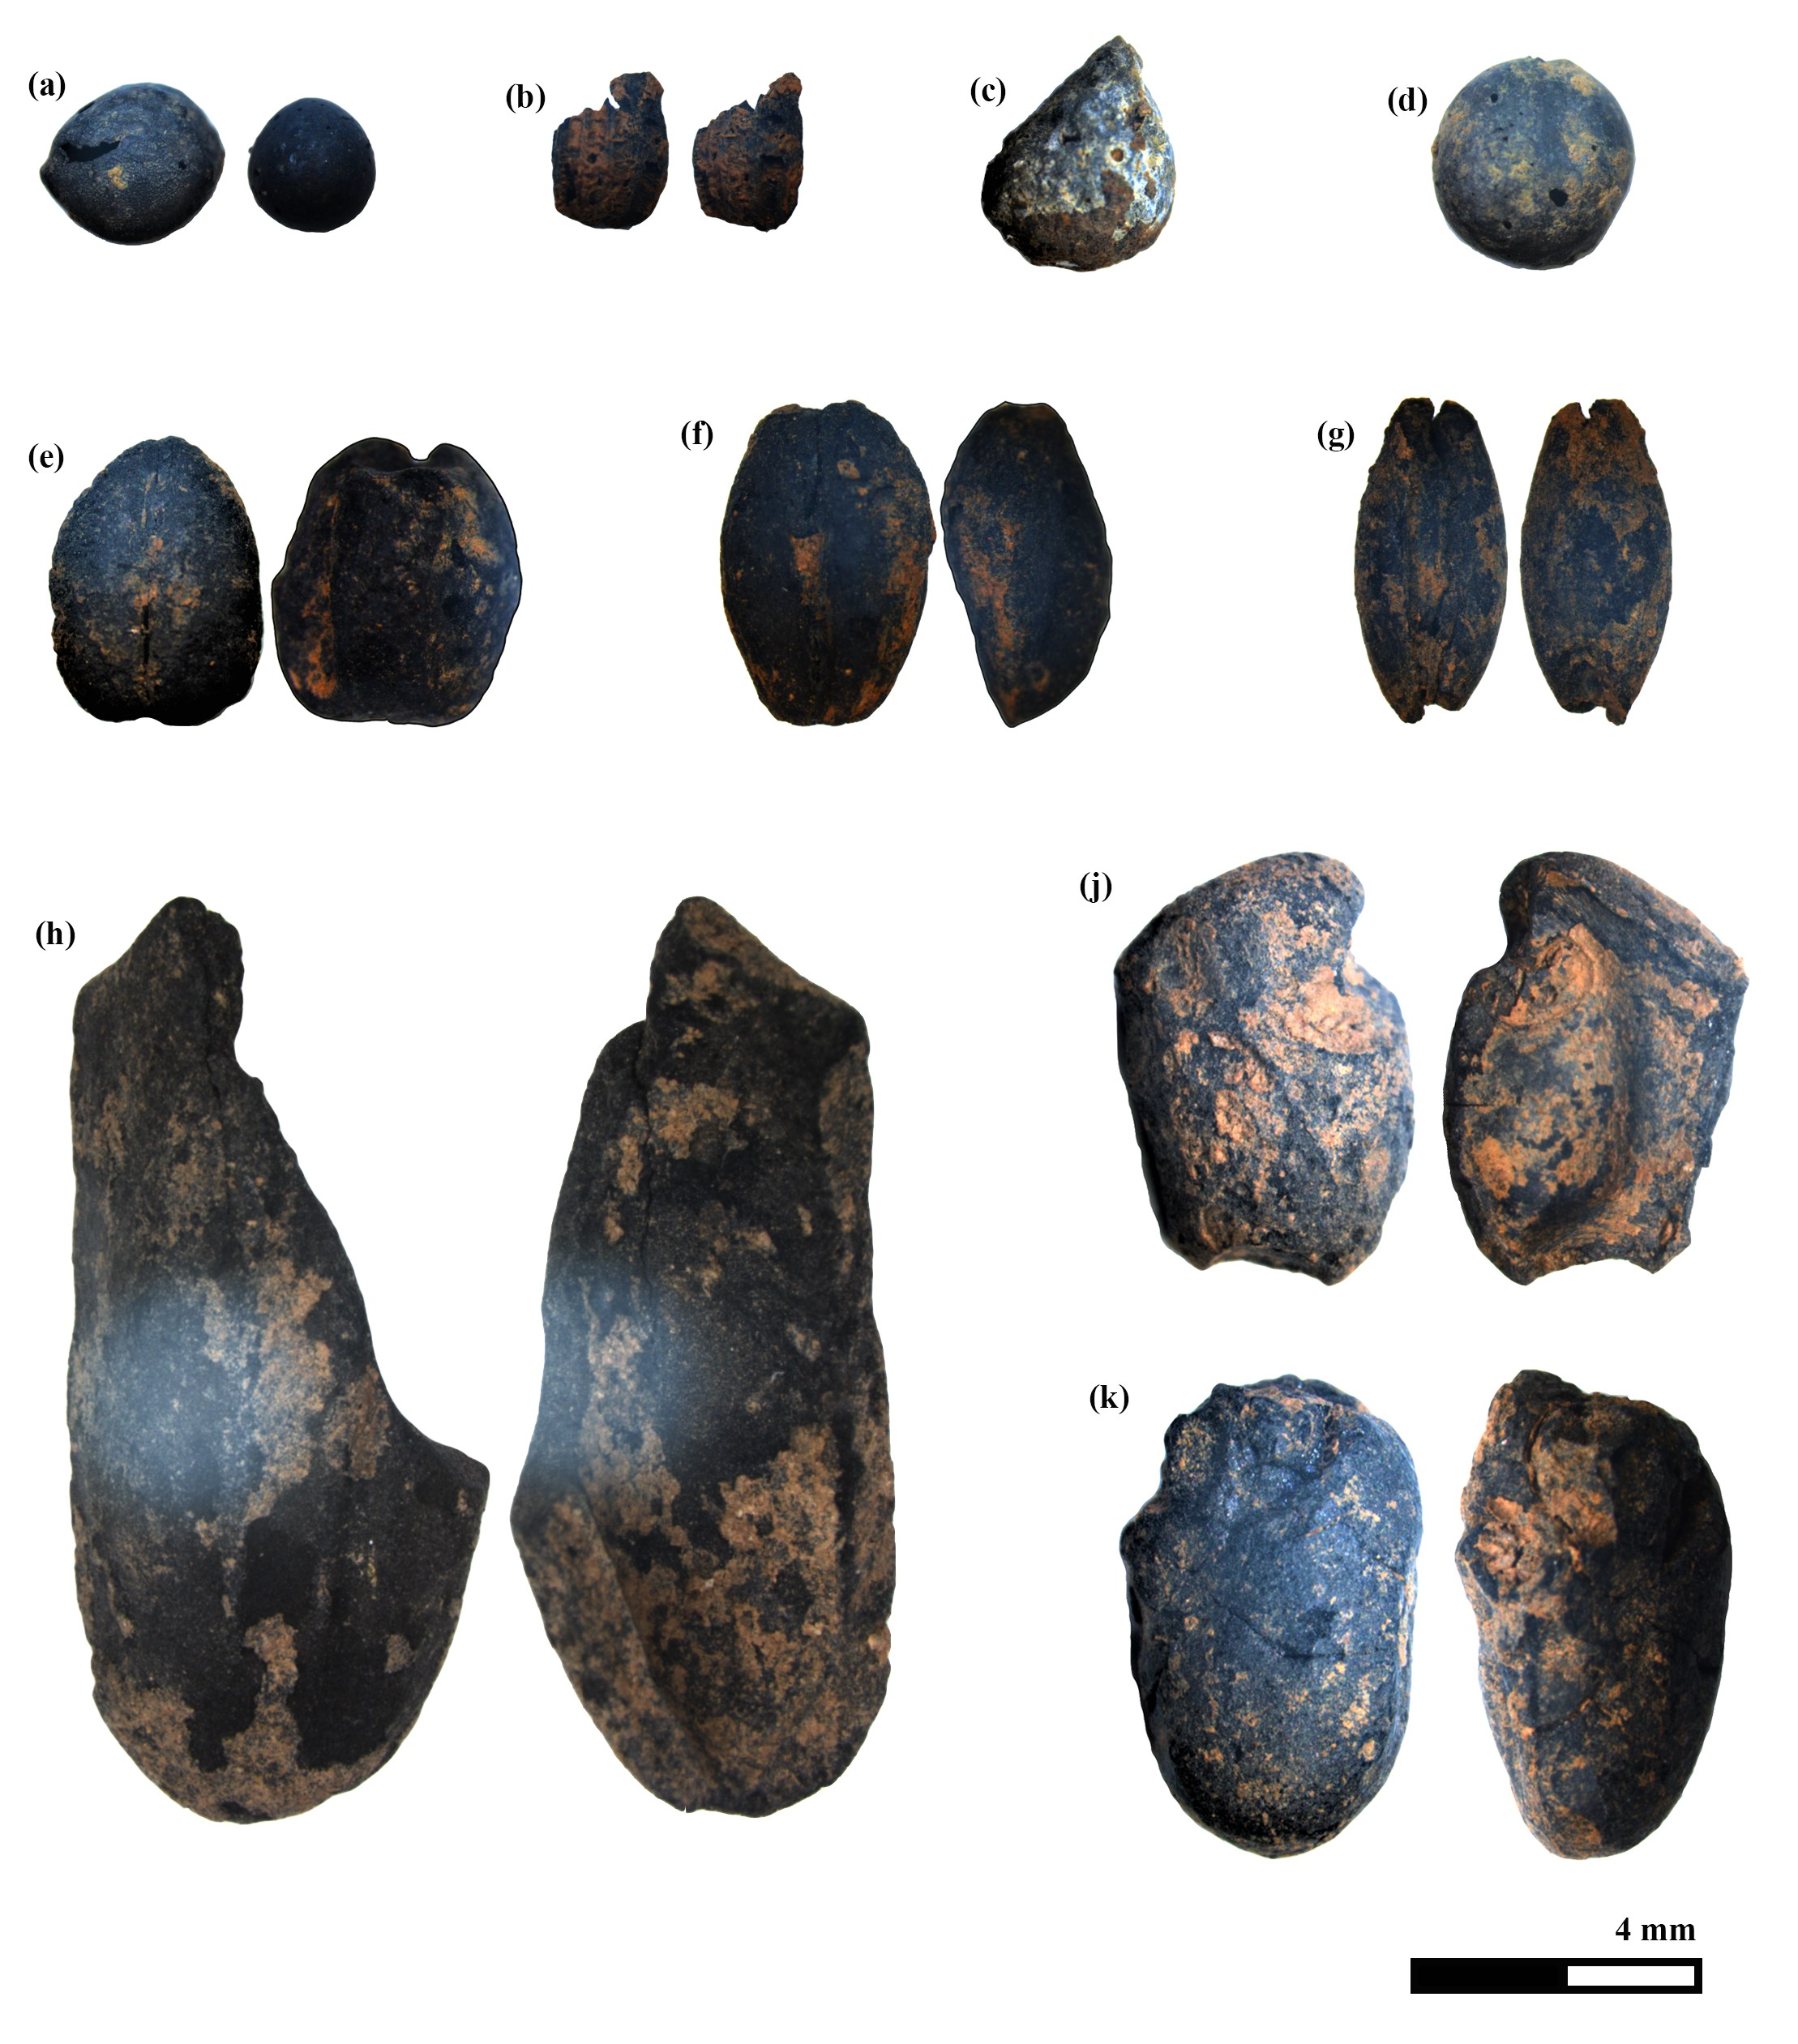
\includegraphics[width=0.98\textwidth]{C:/Users/rosha/Documents/R/Projects/castro_marim_phoenician/./images/castro_bot_assemblage} \caption{Charred botanical remains of settlement phase V from Castro Marim; \textbf{(a)} \emph{Brassica nigra}; \textbf{(b)} \emph{Apium} sp.; \textbf{(c)} \emph{Galeopsis tetrahit}; \textbf{(d)} \emph{Pisum sativum}; \textbf{(e)} \emph{Triticum aestivum/durum}; \textbf{(f)} \emph{Hordeum vulgare nudum}; \textbf{(g)} \emph{Hordeum vulgare vulgare}; \textbf{(h)} \emph{Pinus} sp.; \textbf{(i)} \emph{Vicia faba}}\label{fig:castro-archbot-assemblage}
\end{figure*}

\hypertarget{results-and-discussion}{%
\section{Results and Discussion}\label{results-and-discussion}}

\hypertarget{bone-preservation}{%
\subsection{Bone Preservation}\label{bone-preservation}}

\hypertarget{fourier-transform---infrared-spectroscopy}{%
\subsubsection{Fourier Transform - Infrared Spectroscopy}\label{fourier-transform---infrared-spectroscopy}}

The IRSF index values are in a range of 2.37 - 3.37 (accepted range is 2.96 - 4.04) and the C/P index values are in the range of 0.2-0.428 (accepted range is 0.054 - 0.47) which fall well within the accepted range for well-preserved archaeological bones (Hollund et al., 2013; Lebon et al., 2016).

\hypertarget{collagen-quality}{%
\subsubsection{Collagen Quality}\label{collagen-quality}}

Collagen extraction was successful for all the bone samples, based on published criteria, with carbon content between 15.3\% and 47.0\% (Ambrose, 1990), nitrogen content between 5.5\% and 17.3\% (Ambrose, 1990), C/N values between 2.9 and 3.6 (DeNiro, 1985), C/S values between 300\% and 900\% (Nehlich and Richards, 2009), and collagen yields greater than 1\% (Klinken, 1999). The extracted bone collagen samples exhibit C/N values ranged between 3.1 and 3.5 and C/S values between 225.9 and 688.4. Carbon and nitrogen amounts range from 20.3\% to 50.0\% and 7.3\% and 18.1\% respectively. Collagen yields range between 2.5\% to 49.1\%. All the faunal samples exhibited collagen quality parameters indicative of good preservation.





\begin{table*}

\caption{\label{tab:table3}\(\delta ^{13}C\) and \(\delta ^{15}N\) values of the two charred \emph{Hordeum vulgare} cultivars.}
\centering
\fontsize{7.5}{9.5}\selectfont
\begin{tabu} to \linewidth {>{\raggedright}X>{}c>{\raggedleft}X>{\raggedright}X>{\raggedright}X>{\raggedright}X>{\raggedright}X>{\raggedright}X>{\raggedright}X}
\toprule
Sample ID & Species & \% C & \% N & $\delta^{13}C (\text{\textperthousand})$ & $\delta^{15}N (\text{\textperthousand})$ & $\delta^{13}C_{corr} (\text{\textperthousand}) ^{*}$ & $\delta^{15}N_{corr} (\text{\textperthousand}) ^{*}$ & $\Delta^{13}C (\text{\textperthousand})$\\
\midrule
CMHV1 & \em{Hordeum vulgare vulgare} & 37.7 & 2.1 & -22.1 & 9.6 & -22.21 & 9.29 & 16.07\\
CMHV2 & \em{Hordeum vulgare vulgare} & 49.7 & 2.8 & -22.6 & 9.4 & -22.71 & 9.09 & 16.59\\
CMHV3 & \em{Hordeum vulgare vulgare} & 50.0 & 2.2 & -24.7 & 9.1 & -24.81 & 8.79 & 18.78\\
CMHN1 & \em{Hordeum vulgare nudum} & 49.1 & 3.6 & -23.0 & 8.9 & -23.11 & 8.59 & 17.00\\
CMHN2 & \em{Hordeum vulgare nudum} & 49.5 & 3.9 & -23.2 & 8.4 & -23.31 & 8.09 & 17.21\\
CMHN3 & \em{Hordeum vulgare nudum} & 47.6 & 2.6 & -23.1 & 9.8 & -23.21 & 9.49 & 17.11\\
\bottomrule
\multicolumn{9}{l}{\rule{0pt}{1em}\textsuperscript{*} \(\delta ^{13}C\) and \(\delta ^{15}N\) values corrected for charring effect.}\\
\end{tabu}
\end{table*}

\begingroup\fontsize{7.5}{9.5}\selectfont

\begin{longtable}[t]{c>{}cccccccccc}
\caption{\label{tab:table4}Carbon, nitrogen, and sulphur isotope composition of the fauna.}\\
\toprule
Sample ID & Species & \% C & \% N & \% S & C:N & C:S & N:S & $\delta^{13}C (\text{\textperthousand})$ & $\delta^{15}N (\text{\textperthousand})$ & $\delta^{34}S (\text{\textperthousand})$\\
\midrule
\endfirsthead
\caption[]{\label{tab:table4}Carbon, nitrogen, and sulphur isotope composition of the fauna. \textit{(continued)}}\\
\toprule
Sample ID & Species & \% C & \% N & \% S & C:N & C:S & N:S & $\delta^{13}C (\text{\textperthousand})$ & $\delta^{15}N (\text{\textperthousand})$ & $\delta^{34}S (\text{\textperthousand})$\\
\midrule
\endhead

\endfoot
\bottomrule
\endlastfoot
CMOF435 & \em{Bos taurus} & 41.1 & 14.9 & 0.2 & 3.2 & 477.5 & 88.9 & -20.2 & 8.9 & 10.3\\
CMOF397 & \em{Capra hircus} & 38.7 & 14.2 & 0.2 & 3.2 & 688.4 & 64.5 & -19.8 & 4.2 & 10.9\\
CMOF388 & \em{Cervus elaphus} & 28.3 & 10.3 & 0.2 & 3.2 & 504.4 & 62.6 & -20.0 & 4.1 & 15.6\\
CMOF424 & \em{Ovis aries} & 40.6 & 14.8 & 0.2 & 3.2 & 493.1 & 73.3 & -20.7 & 7.0 & 7.7\\
CMOF230 & \em{Oryctolagus cuniculus} & 40.9 & 14.9 & 0.3 & 3.2 & 436.8 & 43.3 & -21.6 & 4.7 & 16.7\\
CMOF181 & \em{Capra hircus} & 41.3 & 15.3 & 0.2 & 3.2 & 580.4 & 59.5 & -19.8 & 4.9 & 12.6\\
CMOF158 & \em{Sus scrofa} & 41.0 & 15.2 & 0.2 & 3.2 & 521.0 & 119.5 & -19.3 & 11.0 & 14.6\\
CMOF779 & \em{Pluvialis squatarola} & 40.8 & 14.8 & 0.3 & 3.2 & 375.9 & 81.6 & -14.9 & 10.3 & 9.5\\
CMOF370 & \em{Bos taurus} & 39.8 & 14.6 & 0.2 & 3.2 & 443.1 & 66.7 & -21.2 & 7.0 & 15.2\\
CMOF373 & \em{Cervus elaphus} & 41.3 & 15.2 & 0.2 & 3.2 & 524.5 & 39.8 & -20.0 & 3.6 & 16.3\\
CMOF402 & \em{Bos taurus} & 41.8 & 15.8 & -- & 3.1 & -- & -- & -19.0 & 7.6 & --\\
CMOF374 & \em{Ovis aries} & 41.1 & 15.3 & 0.3 & 3.1 & 406.0 & 68.4 & -17.3 & 8.1 & 13.4\\
CMOF254 & \em{Oryctolagus cuniculus} & 40.4 & 14.6 & 0.3 & 3.2 & 385.5 & 96.8 & -21.5 & 11.8 & 11.4\\
CMOF756 & \em{Alectoris rufa} & 41.0 & 15.1 & 0.3 & 3.2 & 438.1 & 53.3 & -20.6 & 5.8 & 13.9\\
CMOF419 & \em{Ovis aries} & 36.8 & 13.5 & 0.2 & 3.2 & 516.5 & 67.1 & -20.8 & 5.6 & 7.0\\
CMOF439 & \em{Sus scrofa} & 21.7 & 8.0 & -- & 3.2 & -- & -- & -19.8 & 8.8 & --\\
CMOF677 & \em{Cervus elaphus} & 41.4 & 14.9 & 0.3 & 3.2 & 394.8 & 31.4 & -20.3 & 3.8 & 15.8\\
CMOF201 & \em{Bos taurus} & 41.9 & 15.6 & 0.2 & 3.1 & 558.6 & 69.4 & -21.4 & 6.1 & 8.3\\
CMOF420 & \em{Capra hircus} & 40.7 & 15.1 & 0.2 & 3.2 & 494.3 & 59.4 & -19.3 & 5.7 & 13.6\\
CMOF463 & \em{Ovis aries} & 40.7 & 15.3 & 0.2 & 3.1 & 543.5 & 86.6 & -20.8 & 7.6 & 15.9\\
CMOF480 & \em{Bos taurus} & 39.1 & 14.4 & 0.2 & 3.2 & 580.6 & 52.5 & -21.7 & 4.1 & 15.3\\
CMOF673 & \em{Capra hircus} & 20.3 & 7.3 & 0.2 & 3.3 & 225.9 & 51.9 & -19.2 & 5.4 & 14.8\\
CMOF660 & \em{Capra hircus} & 42.3 & 15.6 & 0.2 & 3.2 & 564.3 & 48.5 & -19.8 & 4.2 & 12.8\\
CMOF656 & \em{Ovis aries} & 40.9 & 15.2 & 0.2 & 3.1 & 574.2 & 46.8 & -19.8 & 3.9 & 17.3\\
CMOF260 & \em{Ovis aries} & 42.5 & 15.9 & -- & 3.1 & -- & -- & -19.8 & 5.9 & --\\
CMOF147 & \em{Bos taurus} & 43.0 & 16.2 & -- & 3.1 & -- & -- & -20.0 & 7.2 & --\\
CMOF354 & \em{Sus scrofa} & 40.9 & 15.3 & 0.2 & 3.1 & 496.0 & 133.8 & -18.0 & 12.9 & 11.4\\
CMOF253 & \em{Sus scrofa} & 40.3 & 15.0 & 0.2 & 3.1 & 489.3 & 76.3 & -19.6 & 7.3 & 11.9\\
CMOF467 & \em{Cervus elaphus} & 34.4 & 12.8 & 0.2 & 3.1 & 539.9 & 59.3 & -20.0 & 4.4 & 14.3\\
CMOF338 & \em{Sus scrofa} & 40.8 & 15.0 & -- & 3.2 & -- & -- & -20.3 & 8.5 & --\\
CMOF99 & \em{Oryctolagus cuniculus} & 42.9 & 14.4 & 0.2 & 3.5 & 602.2 & 99.9 & -20.5 & 8.3 & 14.3\\
CMOF466 & \em{Sus scrofa} & 40.8 & 15.0 & 0.2 & 3.2 & 544.1 & 100.4 & -20.1 & 8.8 & 14.4\\
CMOF710 & \em{Gallus domesticus} & 40.5 & 14.7 & 0.3 & 3.2 & 415.9 & 81.5 & -18.9 & 9.3 & 16.2\\
CMOF'737 & \em{Alectoris rufa} & 40.6 & 14.9 & 0.3 & 3.2 & 416.8 & 49.0 & -20.0 & 5.6 & 13.9\\
CMOF774 & \em{Gallus domesticus} & 40.7 & 14.9 & 0.2 & 3.2 & 452.9 & 74.4 & -20.2 & 7.8 & 15.1\\
CMOF750 & \em{Gallus domesticus} & 40.6 & 15.1 & 0.2 & 3.1 & 451.9 & 94.8 & -18.2 & 9.9 & 13.5\\
CMOF323 & \em{Sus scrofa} & 40.4 & 14.9 & -- & 3.2 & -- & -- & -20.3 & 7.3 & --\\
CMOF508 & \em{Cervus elaphus} & 38.0 & 14.3 & -- & 3.1 & -- & -- & -20.0 & 3.5 & --\\
CMOF751 & \em{Gallus domesticus} & 40.6 & 14.8 & 0.2 & 3.2 & 515.8 & 106.5 & -18.1 & 9.8 & 14.9\\
CMOF772 & \em{Gallus domesticus} & 40.7 & 14.9 & 0.2 & 3.2 & 452.8 & 91.1 & -18.5 & 9.6 & 14.9\\
CMOF743 & \em{Gallus domesticus} & 41.1 & 15.0 & 0.2 & 3.2 & 498.4 & 100.2 & -18.1 & 9.6 & 12.5\\
CMOF14 & \em{Capra hircus} & 36.6 & 13.1 & -- & 3.3 & -- & -- & -20.3 & 3.9 & --\\
CMOF777 & \em{Rissa tridactyla} & 40.9 & 15.1 & 0.3 & 3.2 & 376.9 & 109.7 & -15.5 & 13.9 & 15.8\\
CMOF691 & \em{Ovis aries} & 40.9 & 15.4 & 0.2 & 3.1 & 545.9 & 106.4 & -20.7 & 9.3 & 12.4\\
CMOF457 & \em{Oryctolagus cuniculus} & 40.5 & 15.0 & 0.2 & 3.2 & 450.9 & 41.3 & -23.2 & 4.3 & 14.2\\
CMOF468 & \em{Bos taurus} & 40.9 & 15.5 & 0.2 & 3.1 & 642.4 & 122.8 & -21.6 & 9.1 & 11.6\\
CMOF746 & \em{Gallus domesticus} & 42.4 & 15.8 & 0.2 & 3.1 & 514.6 & 100.4 & -17.3 & 9.6 & 12.2\\
CMOF744 & \em{Gallus domesticus} & 43.4 & 16.0 & 0.3 & 3.2 & 429.3 & 80.1 & -17.5 & 9.5 & 14.7\\
CMOF731 & \em{Gallus domesticus} & 42.8 & 15.6 & 0.3 & 3.2 & 393.6 & 86.0 & -19.3 & 10.9 & 16.2\\
CMOF730 & \em{Gallus domesticus} & 50.0 & 18.1 & 0.2 & 3.2 & 606.3 & 115.5 & -19.6 & 11.1 & 14.1\\
CMOF709 & \em{Gallus domesticus} & 42.8 & 15.7 & 0.2 & 3.2 & 544.0 & 119.8 & -18.7 & 11.0 & 14.6\\
CMOF643 & \em{Cervus elaphus} & 42.8 & 15.9 & -- & 3.1 & -- & -- & -19.7 & 2.9 & --\\
CMOF504 & \em{Cervus elaphus} & 38.6 & 13.9 & -- & 3.2 & -- & -- & -19.8 & 3.4 & --\\
CMOF477 & \em{Ovis aries} & 43.9 & 15.6 & 0.2 & 3.3 & 558.3 & 61.0 & -19.5 & 5.6 & 8.8\\
CMOF394 & \em{Capra hircus} & 27.2 & 10.0 & 0.2 & 3.2 & 426.9 & 85.7 & -19.6 & 6.4 & 9.2\\
CMOF393 & \em{Bos taurus} & 42.1 & 15.3 & -- & 3.2 & -- & -- & -20.3 & 3.9 & --\\
CMOF353 & \em{Oryctolagus cuniculus} & 42.7 & 15.8 & 0.2 & 3.2 & 495.4 & 110.2 & -21.0 & 11.1 & 12.6\\
CMOF334 & \em{Oryctolagus cuniculus} & 43.3 & 15.9 & -- & 3.2 & -- & -- & -20.6 & 11.2 & --\\
CMOF324 & \em{Oryctolagus cuniculus} & 43.9 & 15.4 & -- & 3.3 & -- & -- & -22.9 & 4.0 & --\\
CMOF303 & \em{Ovis aries} & 42.1 & 15.7 & 0.2 & 3.1 & 562.5 & 80.0 & -20.2 & 7.0 & 9.6\\
CMOF94 & \em{Bos taurus} & 36.7 & 13.9 & 0.2 & 3.1 & 490.4 & 58.0 & -20.9 & 5.1 & 7.8\\
CMOF745 & \em{Gallus domesticus} & 41.0 & 15.3 & 0.2 & 3.1 & 476.1 & 95.2 & -18.2 & 9.6 & 15.2\\*
\end{longtable}
\endgroup{}

\hypertarget{botanical-remains}{%
\subsection{Botanical Remains}\label{botanical-remains}}

No botanical remains could be recovered from the soil samples of phases I -- IV due to the smaller scale of settlements as well as poor preservation conditions. The bulk of the recovered remains are from phase V representing the most mature chronological period of the occupation. Barley (\emph{Hordeum vulgare}) is the most dominant taxon in the botanical record (Table \ref{tab:table2}). \emph{Hordeum vulgare nudum} and \emph{Hordeum vulgare vulgare} (Fig. \ref{fig:castro-archbot-assemblage} \textbf{(f)} and \textbf{(g)} respectively) are the two cultivars which constitute the barley fraction with equal abundance. Wheat (\emph{Triticum aestivum}) is second most abundant taxon after barley. Large scale cereal cultivation has been observed in sites located in river valleys near South Iberian sea coast (Eg: Castillo de Doña Blanca (Guadalquivir Valley, Spain) and El Villar (Guadalhorce valley, Spain), two sites which are located in similar geographical settings to Castro Marim). Cereal cultivation seems to be a major activity with implication being that cereals were the principle source of carbohydrates for both humans and animals. The greater presence of barley compared to wheat can be a strategy of `minimum returns on investment' against dry climatic conditions exploiting the fact that barley has higher tolerance to drier conditions compared to wheat (Riehl, 2009). Two taxa of leguminous plants have been noted namely, peas (\emph{Pisum sativum}) and broad bean (\emph{Vicia faba}) (Fig. \ref{fig:castro-archbot-assemblage} \textbf{(d)} and \textbf{(i)} respectively). The leguminous plants serve as a rich source of proteins and act as an alternate to animal sourced protein for humans. The combined cultivation of leguminous plants with cereals helps maintain adequate soil nitrogen levels, leading to a sustainable and diverse production. The presence of black mustard (\emph{Brassica nigra}) (Fig. \ref{fig:castro-archbot-assemblage} \textbf{(a)}) has been recorded. Black mustard is a common species along the rocky Mediterranean coasts and have long found their place as a culinary taste enhancer (Dixon, 2006). Like many members of \emph{Brassica}, black mustard was also used as a source of oil. A fragment of a charred seed has been attributed to \emph{Apium} taxon, suspected to be a seed of celery (\emph{Apium graveolens}) (Fig. \ref{fig:castro-archbot-assemblage} \textbf{(b)}). This attribution is done due to the presence of five slender longitudinal ridges on the surface of the seed (Wilson, 2016). The species is native to the coastal Mediterranean region, considered to be its centre of origin. The recorded use of celery as a vegetable in Europe is only from the 1600s, originating in Italy, with gradual spread westwards in the subsequent centuries (Tobyn et al., 2011). Hortulus, a Strabo poem from 9th century B.C.E describes the use of celery as a medicinal plant implying that even if the plant was cultivated as a medicinal herb rather than as a food plant (Sturtevant, 1886) in the Phoenician - Punic period. Shells of pine nuts (\emph{Pinus} sp.) (Fig. \ref{fig:castro-archbot-assemblage} \textbf{(h)}) are suspected to be from the \emph{Pinus pinea} species, commonly known as Mediterranean stone pine. Pine nut consumption has been documented in Portugal since Palaeolithic period (Gale and Carruthers, 2000). The nuts of stone pine are high in protein ansd fat with low carbohydrates (Haws, 2004). The nuts are a valuable source of nutrition and could have been stored to deal with periods of low cultivated food production.



\begin{figure}
\centering
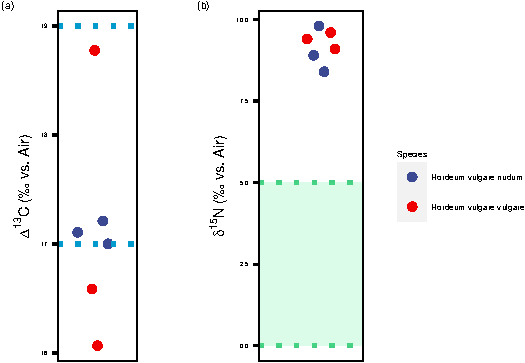
\includegraphics{castro_main_body_files/figure-latex/iso-hord-plots-1.pdf}
\caption{\label{fig:iso-hord-plots}\textbf{(a).} Beeswarm plot showing \(\Delta ^{13}C\) values of barley cultivars where the blue dashed lines represent `well-watered,' `moderately-watered,' and `poorly watered' reference lines based on the study of modern crops in varying watering conditions (Wallace et al., 2013). \textbf{(b).} Beeswarm plot showing the manuring status of barley cultivars with green shaded region representing 1 SD range of estimated wild herbivore forage value (calculated from subtraction 4 \permil from red deer \(\delta ^{15}N\) mean ± 1 SD range).}
\end{figure}

\hypertarget{watering-regimes-and-manuring-intensity-of-barley}{%
\subsection{Watering regimes and manuring intensity of barley}\label{watering-regimes-and-manuring-intensity-of-barley}}

Table \ref{tab:table3}. shows the results of stable isotope results of the two barley cultivars. The isotope measurements fall within the established predicted ranges obtained from experimentally charred modern cereals (Fraser et al., 2013). The \(\delta ^{13}C\) values are within the range expected for a C\textsubscript{3} plant with \emph{Hordeum vulgare nudum} having a mean of -23.21 ± 0.1\permil, while that of \emph{Hordeum vulgare vulgare} is -23.24 ± 1.38\permil. The \(\delta ^{13}C\) means of both cultivars show no statistically significant difference (t-statistic: -0.04, degrees of freedom: 4, \emph{p}-value: 0.97). The \(\Delta ^{13}C\) values (Figure \ref{fig:iso-hord-plots} \textbf{(a)}) show barley cultivated in a poor to moderate watering conditions which would indicate that the plants have been dependant on natural precipitation with little or no artificial irrigation. The barley however was not growing in water deficit conditions since Castro Marim is surrounded by marshlands, being on the Guadiana estuary. Both the cultivars exhibit high \(\delta ^{15}N\) values (\emph{Hordeum vulgare nudum}, 8.72 ± 0.71\permil; \emph{Hordeum vulgare vulgare} a mean of 9.06 ± 0.25\permil) with no significant difference (t-statistic: 0.77, degrees of freedom: 4, \emph{p}-value: 0.49). The \(\delta ^{15}N\) values indicate high manuring intensity which is consequential due to the close proximity of the agricultural plots to the settlement and the river. The lack of artificial irrigation with relatively intense manuring of barley at Castro Marim indicates a strategy of minimal effort and risk while ensuring optimal produce.

\hypertarget{faunal-bone-collagen-delta-13c-and-delta-15n-values}{%
\subsection{\texorpdfstring{Faunal bone collagen \(\delta ^{13}C\) and \(\delta ^{15}N\) values}{Faunal bone collagen \textbackslash delta \^{}\{13\}C and \textbackslash delta \^{}\{15\}N values}}\label{faunal-bone-collagen-delta-13c-and-delta-15n-values}}



\begin{figure}
\centering
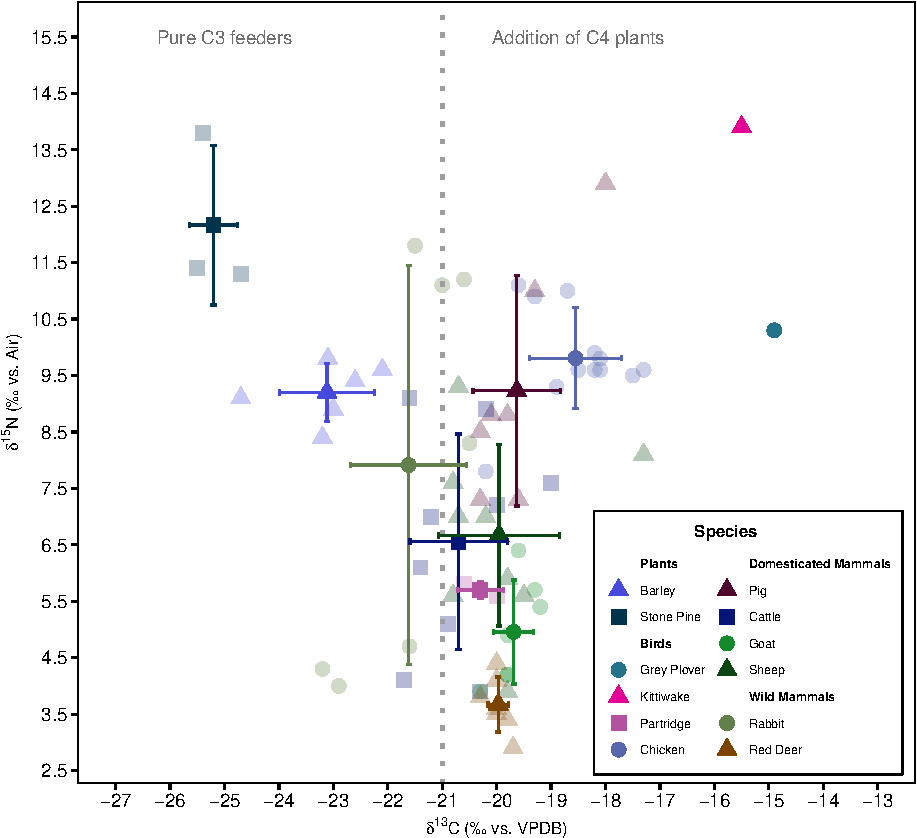
\includegraphics{castro_main_body_files/figure-latex/fauna-carbnitro-iso-plot-1.pdf}
\caption{\label{fig:fauna-carbnitro-iso-plot}Plot showing mean \(\delta ^{13}C\) and \(\delta ^{15}N\) values of faunal bone collagen.}
\end{figure}



\begin{figure*}
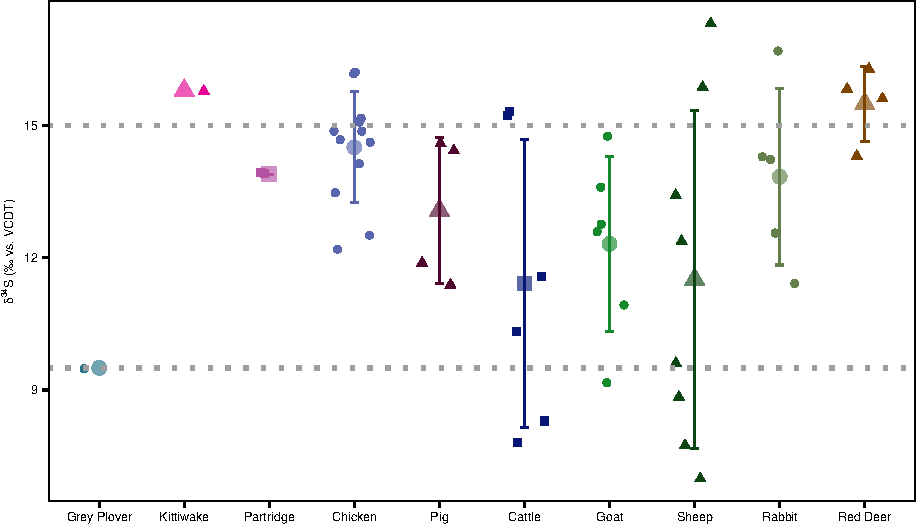
\includegraphics[width=0.98\textwidth]{castro_main_body_files/figure-latex/fauna-sulph-iso-plot-1} \caption{Plot showing mean \(\delta ^{34}S\) values of faunal bone collagen.}\label{fig:fauna-sulph-iso-plot}
\end{figure*}

All fifty faunal samples with the exception of rabbits (in case of \(\delta ^{15}N\)), demonstrate (Table \ref{tab:table4}) stable isotope values within the range expected for a C\textsubscript{3} temperate ecosystem. The mean \(\delta ^{13}C\) and \(\delta ^{15}N\) values of red deer are -19.97 ± 0.19\permil and 3.67 ± 0.49\permil respectively. The other undomesticated specie is the rabbit which has mean \(\delta ^{13}C\) values of -21.61 ± 1.07\permil and mean \(\delta ^{15}N\) values of 7.91 ± 3.53\permil. The mean \(\delta ^{13}C\) values of red deer are significantly higher than those of rabbit (t-statistic: -4.01, degrees of freedom: 12, \emph{p}-value: 0). This can attributed to the foraging area of the rabbits which is usually at the ground level with high recycling of CO\textsubscript{2} and shade from the higher levels of the canopy. The \(\delta ^{15}N\) values of rabbits are anomalous with a standard deviation spanning almost a trophic level. This large spread of \(\delta ^{15}N\) values is explained in section \ref{sulphur}.

Sheep show mean \(\delta ^{13}C\) values of -19.96 ± 1.11\permil and mean \(\delta ^{15}N\) values of 6.67 ± 1.6\permil, while goats exhibit mean \(\delta ^{13}C\) values of -19.69 ± 0.37\permil and mean \(\delta ^{15}N\) values of 4.96 ± 0.92\permil. Goat mean \(\delta ^{13}C\) values are not significantly different than that of sheep (t-statistic: 0.61, degrees of freedom: 14, \emph{p}-value: 0.55). Sheep also exhibit significantly higher \(\delta ^{15}N\) values than goats (t-statistic: 2.5, degrees of freedom: 14, \emph{p}-value: 0.03) which demonstrates that sheep were fed on food sourced from manured vegetation. Sheep are superior to goats both in terms of secondary products and ease of management (Davis, 2007; Rutter, 2002). Owing to the more attached economic interests with sheep, it is natural to give food sourced from cultivated crops.
Cattle show mean \(\delta ^{13}C\) values of -20.7 ± 0.89\permil and mean \(\delta ^{15}N\) values of 6.56 ± 1.91\permil. Most of the cattle bones are from adults indicative that they were used as a source of power and only slaughtered for meat towards the end of their life (Davis, 2007). The cattle seem to have grazed in a more forested area in contrast to ovicaprines feeding in open pastures.Feeding in forested areas causes the \(\delta ^{13}C\) values to increase due to canopy effect (Bonafini et al., 2013). Pigs show mean \(\delta ^{13}C\) values of -19.63 ± 0.81\permil and mean \(\delta ^{15}N\) values of 9.23 ± 2.04\permil. The high \(\delta ^{15}N\) values of pigs, reflect an omnivorous diet. The pigs could have been penned in spaces attached to human residences, giving rise to the possibility to be fed remnants of human diet. Partridges show mean \(\delta ^{13}C\) values of -20.3 ± 0.42\permil and mean \(\delta ^{15}N\) values of 5.7 ± 0.14\permil while chicken exhibit mean \(\delta ^{13}C\) values of -18.55 ± 0.84\permil and mean \(\delta ^{15}N\) values of 9.81 ± 0.9\permil. The \(\delta ^{13}C\) values (t-statistic: 2.8, degrees of freedom: 12, \emph{p}-value: 0.02) and \(\delta ^{15}N\) values (t-statistic: 6.26, degrees of freedom: 12, \emph{p}-value: \ensuremath{4\times 10^{-5}}) are significantly different. The chicken owing to its domesticated status has higher \(\delta ^{13}C\) and \(\delta ^{15}N\) values. Chickens are usually reared in domestic spaces while being fed food scraps and possibly fed millet (a C\textsubscript{4} plant) (Fernández-Crespo et al., 2019). Chicken also eat insects alongside the human provided food which can lead to an increase of \(\delta ^{15}N\) values. All the partridges recovered are adults whereas the chickens constitute juvenile-adult mix, further indicative that the former were hunted for human consumption.

High mean \(\delta ^{13}C\) and \(\delta ^{15}N\) values (Fig. \ref{fig:fauna-carbnitro-iso-plot}) of domesticates can be obtained by rearing the animals in either domestic spaces or harvested fields, while feeding them cultivated crops (cereals) and associated by-products in the animal feed along with the natural wild flora. The \(\delta ^{13}C\) values of wild species are indicative of a diet from forested areas with vegetation having lower \(\delta ^{15}N\) values than cultivated crops.

\hypertarget{sulphur}{%
\subsection{\texorpdfstring{Faunal bone collagen \(\delta ^{34}S\) values}{Faunal bone collagen \textbackslash delta \^{}\{34\}S values}}\label{sulphur}}

\hypertarget{conclusions}{%
\section{Conclusions}\label{conclusions}}

\hypertarget{references}{%
\section*{References}\label{references}}
\addcontentsline{toc}{section}{References}

\hypertarget{refs}{}
\begin{CSLReferences}{1}{0}
\leavevmode\hypertarget{ref-ambrose90}{}%
Ambrose, S.H., 1990. Preparation and characterization of bone and tooth collagen for isotopic analysis. Journal of Archaeological Science 17, 431--451. doi:\href{https://doi.org/10.1016/0305-4403(90)90007-R}{10.1016/0305-4403(90)90007-R}

\leavevmode\hypertarget{ref-arrastio99}{}%
Arrastio, F.J.M., 1999. Conflictos y perspectivas en el periodo precolonial tartésico. Gerión. Revista de Historia Antigua 17, 149.

\leavevmode\hypertarget{ref-arrastio00}{}%
Arrastio, F.J.M., 2000. Tartessos, estelas, modelos pesimistas, in: Intercambio y Comercio Preclásico En El {Mediterráneo}: Actas Del {I} Coloquio Del {CEFYP}, {Madrid}, 9-12 de Noviembre, 1998. {Centro de Estudios Fenicios y Púnicos}, pp. 153--174.

\leavevmode\hypertarget{ref-arruda96}{}%
Arruda, A.M., 1996. O {Castelo} de {Castro Marim}, in: In {De Ulisses} a {Viriato}. {O} Primeiro Milénio a.{C}.. {Ministério da Cultura, Instituto Português de Museus, Museu Nacional de Arqueologia}, {Lisboa}, pp. 95--100.

\leavevmode\hypertarget{ref-arruda03}{}%
Arruda, A.M., 2003. Contributo da colonização fenícia para a domesticação da terra portuguesa. Ecohistoria del paisaje agrario-la agricultura fenicio-púnica en el mediterráneo.

\leavevmode\hypertarget{ref-arruda09}{}%
Arruda, A.M., 2009. Phoenician colonization on the {Atlantic Coast} of the {Iberian Peninsula}. {Chicago: The University of Chicago Press, 2009.}

\leavevmode\hypertarget{ref-arruda_freitas08}{}%
Arruda, A.M., Freitas, V.T. de, 2008. O castelo de castro marim durante os séculos VI e v a.n.e. Sidereum Ana I: El río Guadiana en época Post-Orientalizante. 429--446.

\leavevmode\hypertarget{ref-arruda_etal13}{}%
Arruda, A.M., Soares, A.M., Freitas, V.T. de, Oliveira, C.F., Martins, J.M.M., Portela, P.J., 2013. A cronologia relativa e absoluta da ocupação sidérica do {Castelo} de {Castro Marim}. Saguntum 45, 101--114.

\leavevmode\hypertarget{ref-arruda_etal06}{}%
Arruda, A.M., Viegas, C., Bargão, P., Pereira, R., 2006. A importação de preparados de peixe em {Castro Marim}: Da {Idade} do {Ferro} á {Época Romana}. Setúbal Arqueológica 13, 153--176.

\leavevmode\hypertarget{ref-aubet01}{}%
Aubet, M.E., 2001. The {Phoenicians} and the {West}: Politics, colonies and trade. {Cambridge Univ. Press}.

\leavevmode\hypertarget{ref-boessneck_etal64}{}%
Boessneck, J., Müller, H.-H., Teichert, M., 1964. Osteologische {Unterscheidungsmerkmale} zwischen {Schaf} ({Ovis} aries {Linné}) und {Ziege} ({Capra} hircus {Linné}). {Verlag nicht ermittelbar}.

\leavevmode\hypertarget{ref-bogaard_etal13}{}%
Bogaard, A., Fraser, R., Heaton, T.H.E., Wallace, M., Vaiglova, P., Charles, M., Jones, G., Evershed, R.P., Styring, A.K., Andersen, N.H., Arbogast, R.-M., Bartosiewicz, L., Gardeisen, A., Kanstrup, M., Maier, U., Marinova, E., Ninov, L., Schäfer, M., Stephan, E., 2013. Crop manuring and intensive land management by {Europe}'s first farmers. PNAS 110, 12589--12594. doi:\href{https://doi.org/10.1073/pnas.1305918110}{10.1073/pnas.1305918110}

\leavevmode\hypertarget{ref-bogaard_etal07}{}%
Bogaard, A., Heaton, T.H.E., Poulton, P., Merbach, I., 2007. The impact of manuring on nitrogen isotope ratios in cereals: Archaeological implications for reconstruction of diet and crop management practices. Journal of Archaeological Science 34, 335--343. doi:\href{https://doi.org/10.1016/j.jas.2006.04.009}{10.1016/j.jas.2006.04.009}

\leavevmode\hypertarget{ref-bonafini_etal13}{}%
Bonafini, M., Pellegrini, M., Ditchfield, P., Pollard, A.M., 2013. Investigation of the 'canopy effect' in the isotope ecology of temperate woodlands. Journal of Archaeological Science 40, 3926--3935. doi:\href{https://doi.org/10.1016/j.jas.2013.03.028}{10.1016/j.jas.2013.03.028}

\leavevmode\hypertarget{ref-buckley_etal10}{}%
Buckley, M., Whitcher Kansa, S., Howard, S., Campbell, S., Thomas-Oates, J., Collins, M., 2010. Distinguishing between archaeological sheep and goat bones using a single collagen peptide. Journal of Archaeological Science 37, 13--20. doi:\href{https://doi.org/10.1016/j.jas.2009.08.020}{10.1016/j.jas.2009.08.020}

\leavevmode\hypertarget{ref-davis07}{}%
Davis, S., 2007. The mammals and birds from the {Iron Age} and {Roman} periods of {Castro Marim}, {Algarve}, {Portugal}. Trabalhos do CIPA 107.

\leavevmode\hypertarget{ref-deniro85}{}%
DeNiro, M.J., 1985. Postmortem preservation and alteration of in vivo bone collagen isotope ratios in relation to palaeodietary reconstruction. Nature 317, 806--809. doi:\href{https://doi.org/10.1038/317806a0}{10.1038/317806a0}

\leavevmode\hypertarget{ref-deniro_epstein81}{}%
Deniro, M.J., Epstein, S., 1981. Influence of diet on the distribution of nitrogen isotopes in animals. Geochimica et Cosmochimica Acta 45, 341--351. doi:\href{https://doi.org/10.1016/0016-7037(81)90244-1}{10.1016/0016-7037(81)90244-1}

\leavevmode\hypertarget{ref-deniro_epstein78}{}%
DeNiro, M.J., Epstein, S., 1978. Influence of diet on the distribution of carbon isotopes in animals. Geochimica et Cosmochimica Acta 42, 495--506. doi:\href{https://doi.org/10.1016/0016-7037(78)90199-0}{10.1016/0016-7037(78)90199-0}

\leavevmode\hypertarget{ref-dietler09}{}%
Dietler, M., 2009. Colonial encounters in {Iberia} and the {Western Mediterranean}: {An} exploratory framework.

\leavevmode\hypertarget{ref-dixon06}{}%
Dixon, G.R., 2006. Origins and diversity of {Brassica} and its relatives., in: Dixon, G.R. (Ed.), Vegetable Brassicas and Related Crucifers. {CABI}, {Wallingford}, pp. 1--33. doi:\href{https://doi.org/10.1079/9780851993959.0001}{10.1079/9780851993959.0001}

\leavevmode\hypertarget{ref-eshel_etal19}{}%
Eshel, T., Erel, Y., Yahalom-Mack, N., Tirosh, O., Gilboa, A., 2019. Lead isotopes in silver reveal earliest {Phoenician} quest for metals in the west {Mediterranean}. Proc Natl Acad Sci USA 116, 6007. doi:\href{https://doi.org/10.1073/pnas.1817951116}{10.1073/pnas.1817951116}

\leavevmode\hypertarget{ref-farquhar_etal89}{}%
Farquhar, G.D., Ehleringer, J.R., Hubick, K.T., 1989. Carbon {Isotope Discrimination} and {Photosynthesis}. Annu. Rev. Plant. Physiol. Plant. Mol. Biol. 40, 503--537. doi:\href{https://doi.org/10.1146/annurev.pp.40.060189.002443}{10.1146/annurev.pp.40.060189.002443}

\leavevmode\hypertarget{ref-farquhar_etal82}{}%
Farquhar, G., O'Leary, M., Berry, J., 1982. On the {Relationship Between Carbon Isotope Discrimination} and the {Intercellular Carbon Dioxide Concentration} in {Leaves}. Functional Plant Biol. 9, 121. doi:\href{https://doi.org/10.1071/PP9820121}{10.1071/PP9820121}

\leavevmode\hypertarget{ref-fernandez-crespo_etal19}{}%
Fernández-Crespo, T., Ordoño, J., Bogaard, A., Llanos, A., Schulting, R., 2019. A snapshot of subsistence in {Iron Age Iberia}: {The} case of {La Hoya} village. Journal of Archaeological Science: Reports 28, 102037. doi:\href{https://doi.org/10.1016/j.jasrep.2019.102037}{10.1016/j.jasrep.2019.102037}

\leavevmode\hypertarget{ref-ferrio_etal05}{}%
Ferrio, J.P., Araus, J.L., Buxó, R., Voltas, J., Bort, J., 2005. Water management practices and climate in ancient agriculture: Inferences from the stable isotope composition of archaeobotanical remains. Veget Hist Archaeobot 14, 510--517. doi:\href{https://doi.org/10.1007/s00334-005-0062-2}{10.1007/s00334-005-0062-2}

\leavevmode\hypertarget{ref-ferrio_etal07}{}%
Ferrio, J.P., Voltas, J., Alonso, N., Araus, J.L., 2007. Reconstruction of {Climate} and {Crop Conditions} in the {Past Based} on the {Carbon Isotope Signature} of {Archaeobotanical Remains}, in: Terrestrial {Ecology}. {Elsevier}, pp. 319--332. doi:\href{https://doi.org/10.1016/S1936-7961(07)01020-2}{10.1016/S1936-7961(07)01020-2}

\leavevmode\hypertarget{ref-fraser_etal13a}{}%
Fraser, R.A., Bogaard, A., Charles, M., Styring, A.K., Wallace, M., Jones, G., Ditchfield, P., Heaton, T.H.E., 2013. Assessing natural variation and the effects of charring, burial and pre-treatment on the stable carbon and nitrogen isotope values of archaeobotanical cereals and pulses. Journal of Archaeological Science 40, 4754--4766. doi:\href{https://doi.org/10.1016/j.jas.2013.01.032}{10.1016/j.jas.2013.01.032}

\leavevmode\hypertarget{ref-fraser_etal11}{}%
Fraser, R.A., Bogaard, A., Heaton, T., Charles, M., Jones, G., Christensen, B.T., Halstead, P., Merbach, I., Poulton, P.R., Sparkes, D., Styring, A.K., 2011. Manuring and stable nitrogen isotope ratios in cereals and pulses: Towards a new archaeobotanical approach to the inference of land use and dietary practices. Journal of Archaeological Science 38, 2790--2804. doi:\href{https://doi.org/10.1016/j.jas.2011.06.024}{10.1016/j.jas.2011.06.024}

\leavevmode\hypertarget{ref-froehle_etal10}{}%
Froehle, A.W., Kellner, C.M., Schoeninger, M.J., 2010. {FOCUS}: Effect of diet and protein source on carbon stable isotope ratios in collagen: Follow up to {Warinner} and {Tuross} (2009). Journal of Archaeological Science 37, 2662--2670. doi:\href{https://doi.org/10.1016/j.jas.2010.06.003}{10.1016/j.jas.2010.06.003}

\leavevmode\hypertarget{ref-gale_carruthers00}{}%
Gale, R., Carruthers, W., 2000. Charcoal and charred seed remains from {Middle Palaeolithic} levels at {Gorham}'s and {Vanguard Caves}. Neanderthals on the Edge. Oxford: Oxbow Books 207--210.

\leavevmode\hypertarget{ref-gomes_arruda18}{}%
Gomes, F.B., Arruda, A.M., 2018. On the edge of history? {The Early Iron Age} of southern {Portugal}, between texts and archaeology. World Archaeology 50, 764--780. doi:\href{https://doi.org/10.1080/00438243.2019.1604258}{10.1080/00438243.2019.1604258}

\leavevmode\hypertarget{ref-gomezbellard19}{}%
Gómez Bellard, C., 2019. Agriculture, in: The {Oxford Handbook} of {The Phoenician} and {Punic Mediterranean}. {Oxford University Press}, pp. 732--745.

\leavevmode\hypertarget{ref-haws04}{}%
Haws, J., 2004. An {Iberian} perspective on {Upper Paleolithic} plant consumption. Promontoria 2, 49--106.

\leavevmode\hypertarget{ref-hedges_reynard07}{}%
Hedges, R.E.M., Reynard, L.M., 2007. Nitrogen isotopes and the trophic level of humans in archaeology. Journal of Archaeological Science 34, 1240--1251. doi:\href{https://doi.org/10.1016/j.jas.2006.10.015}{10.1016/j.jas.2006.10.015}

\leavevmode\hypertarget{ref-hobson99}{}%
Hobson, K.A., 1999. Tracing origins and migration of wildlife using stable isotopes: A review. Oecologia 120, 314--326. doi:\href{https://doi.org/10.1007/s004420050865}{10.1007/s004420050865}

\leavevmode\hypertarget{ref-hollund_etal13}{}%
Hollund, H.I., Ariese, F., Fernandes, R., Jans, M.M.E., Kars, H., 2013. Testing an {Alternative High}-{Throughput Tool} for {Investigating Bone Diagenesis}: {Ftir} in {Attenuated Total Reflection} (atr) {Mode}*. Archaeometry 55, 507--532. doi:\href{https://doi.org/10.1111/j.1475-4754.2012.00695.x}{10.1111/j.1475-4754.2012.00695.x}

\leavevmode\hypertarget{ref-kellner_schoeninger07}{}%
Kellner, C.M., Schoeninger, M.J., 2007. A simple carbon isotope model for reconstructing prehistoric human diet. American Journal of Physical Anthropology 133, 1112--1127. doi:\href{https://doi.org/10.1002/ajpa.20618}{10.1002/ajpa.20618}

\leavevmode\hypertarget{ref-vanklinken99}{}%
Klinken, G.J. van, 1999. Bone {Collagen Quality Indicators} for {Palaeodietary} and {Radiocarbon Measurements}. Journal of Archaeological Science 26, 687--695. doi:\href{https://doi.org/10.1006/jasc.1998.0385}{10.1006/jasc.1998.0385}

\leavevmode\hypertarget{ref-kohn10}{}%
Kohn, M.J., 2010. Carbon isotope compositions of terrestrial {C3} plants as indicators of (paleo)ecology and (paleo)climate. Proc Natl Acad Sci U S A 107, 19691--19695. doi:\href{https://doi.org/10.1073/pnas.1004933107}{10.1073/pnas.1004933107}

\leavevmode\hypertarget{ref-lebon_etal16}{}%
Lebon, M., Reiche, I., Gallet, X., Bellot-Gurlet, L., Zazzo, A., 2016. Rapid {Quantification} of {Bone Collagen Content} by {ATR}-{FTIR Spectroscopy}. Radiocarbon 58, 131--145. doi:\href{https://doi.org/10.1017/RDC.2015.11}{10.1017/RDC.2015.11}

\leavevmode\hypertarget{ref-leegood13}{}%
Leegood, R.C., 2013. Photosynthesis, in: Lennarz, W.J., Lane, M.D. (Eds.), Encyclopedia of {Biological Chemistry} ({Second Edition}). {Academic Press}, {Waltham}, pp. 492--496. doi:\href{https://doi.org/10.1016/B978-0-12-378630-2.00049-9}{10.1016/B978-0-12-378630-2.00049-9}

\leavevmode\hypertarget{ref-longin71}{}%
Longin, R., 1971. New {Method} of {Collagen Extraction} for {Radiocarbon Dating}. Nature 230, 241--242. doi:\href{https://doi.org/10.1038/230241a0}{10.1038/230241a0}

\leavevmode\hypertarget{ref-lyman94}{}%
Lyman, R.L., 1994. Vertebrate taphonomy. {Cambridge University Press}.

\leavevmode\hypertarget{ref-manfredi92}{}%
Manfredi, L.I., 1992. Le saline et il sale nel mundo punico. Rivista di Studi Fenici 20, 3--14.

\leavevmode\hypertarget{ref-markoe05}{}%
Markoe, G.E., 2005. Phoenicians. {London}: {The British Museum}.

\leavevmode\hypertarget{ref-martin71}{}%
Martin, R., 1971. Recherches sur les agronomes latins et leurs conceptions économiques et sociales.

\leavevmode\hypertarget{ref-nehlich15}{}%
Nehlich, O., 2015. The application of sulphur isotope analyses in archaeological research: {A} review. Earth-Science Reviews 142, 1--17. doi:\href{https://doi.org/10.1016/j.earscirev.2014.12.002}{10.1016/j.earscirev.2014.12.002}

\leavevmode\hypertarget{ref-nehlich_richards09}{}%
Nehlich, O., Richards, M.P., 2009. Establishing collagen quality criteria for sulphur isotope analysis of archaeological bone collagen. Archaeological and Anthropological Sciences 1, 59--75. doi:\href{https://doi.org/10.1007/s12520-009-0003-6}{10.1007/s12520-009-0003-6}

\leavevmode\hypertarget{ref-neville98}{}%
Neville, A., 1998. The {Phoenicians} in {Iberia}: {Settlements}, {Cemetries}, {Trade} and {Agriculture}.

\leavevmode\hypertarget{ref-niemeyer84}{}%
Niemeyer, H.G., 1984. Die {Phönizier} und die {Mittelmeerwelt} im {Zeitalter Homers}. {Jahrbuch des Römisch-Germanischen Zentralmuseums}.

\leavevmode\hypertarget{ref-nitsch_etal15}{}%
Nitsch, E.K., Charles, M., Bogaard, A., 2015. Calculating a statistically robust \(\delta ^{13}C\) and \(\delta ^{15}N\) offset for charred cereal and pulse seeds. STAR: Science \& Technology of Archaeological Research 1, 1--8. doi:\href{https://doi.org/10.1179/2054892315Y.0000000001}{10.1179/2054892315Y.0000000001}

\leavevmode\hypertarget{ref-nitsch_etal19}{}%
Nitsch, E.K., Lamb, A.L., Heaton, T.H.E., Vaiglova, P., Fraser, R., Hartman, G., Moreno-Jiménez, E., López-Piñeiro, A., Peña-Abades, D., Fairbairn, A., Eriksen, J., Bogaard, A., 2019. The {Preservation} and {Interpretation} of {\(\delta^{34}\)S Values} in {Charred Archaeobotanical Remains}. Archaeometry 61, 161--178. doi:\href{https://doi.org/10.1111/arcm.12388}{10.1111/arcm.12388}

\leavevmode\hypertarget{ref-payne69}{}%
Payne, S., 1969. A metrical distinction between sheep and goat metacarpals. The domestication and exploitation of plants and animals 295--305.

\leavevmode\hypertarget{ref-price_etal17}{}%
Price, G.C., Krigbaum, J., Shelton, K., 2017. Stable isotopes and discriminating tastes: {Faunal} management practices at the {Late Bronze Age} settlement of {Mycenae}, {Greece}. Journal of Archaeological Science: Reports 14, 116--126. doi:\href{https://doi.org/10.1016/j.jasrep.2017.05.034}{10.1016/j.jasrep.2017.05.034}

\leavevmode\hypertarget{ref-queiroz_etal06}{}%
Queiroz, P., Mateus, J., Leeuwaarden, W., Pereira, T., Dise, D., 2006. Castro {Marim} e o seu território imediato durante a {Antiguidade}. {Paleo}-etno-{Botânica}. {Relatório Final}. doi:\href{https://doi.org/10.13140/RG.2.2.25361.63848}{10.13140/RG.2.2.25361.63848}

\leavevmode\hypertarget{ref-quinn19}{}%
Quinn, J., 2019. In search of the {Phoenicians}. {Princeton University Press}.

\leavevmode\hypertarget{ref-rcoreteam20}{}%
R Core Team, 2020. R: {A Language} and {Environment} for {Statistical Computing}. {R Foundation for Statistical Computing}, {Vienna, Austria}.

\leavevmode\hypertarget{ref-renzi_etal12}{}%
Renzi, M., Rovira Llorens, S., Montero Ruiz, I., 2012. Riflessioni sulla metallurgia fenicia dell'argento nella {Penisola Iberica}.

\leavevmode\hypertarget{ref-richards_hedges99}{}%
Richards, M.P., Hedges, R.E.M., 1999. Stable {Isotope Evidence} for {Similarities} in the {Types} of {Marine Foods Used} by {Late Mesolithic Humans} at {Sites Along} the {Atlantic Coast} of {Europe}. Journal of Archaeological Science 26, 717--722. doi:\href{https://doi.org/10.1006/jasc.1998.0387}{10.1006/jasc.1998.0387}

\leavevmode\hypertarget{ref-riehl09}{}%
Riehl, S., 2009. Archaeobotanical evidence for the interrelationship of agricultural decision-making and climate change in the ancient {Near East}. Quaternary International 197, 93--114. doi:\href{https://doi.org/10.1016/j.quaint.2007.08.005}{10.1016/j.quaint.2007.08.005}

\leavevmode\hypertarget{ref-roller14}{}%
Roller, D.W., 2014. The geography of {Strabo}: {An English} translation, with introduction and notes. {Cambridge University Press}.

\leavevmode\hypertarget{ref-rutter02}{}%
Rutter, S.M., 2002. Behaviour of {Sheep} and {Goats}, in: The Ethology of Domestic Animals: {An} Introductory Text. pp. 148--155.

\leavevmode\hypertarget{ref-schoeninger85}{}%
Schoeninger, M.J., 1985. Trophic level effects on {15N}/{14N} and {13C}/{12C} ratios in bone collagen and strontium levels in bone mineral. Journal of Human Evolution 14, 515--525. doi:\href{https://doi.org/10.1016/S0047-2484(85)80030-0}{10.1016/S0047-2484(85)80030-0}

\leavevmode\hypertarget{ref-schramm67}{}%
Schramm, Z., 1967. Morphological differences of some goat and sheep bones. {Wyższa Szkoła Rolnicza}.

\leavevmode\hypertarget{ref-sturtevant86}{}%
Sturtevant, E.L., 1886. History of {Celery}. The American Naturalist 20, 599--606. doi:\href{https://doi.org/10.1086/274288}{10.1086/274288}

\leavevmode\hypertarget{ref-tieszen91}{}%
Tieszen, L.L., 1991. Natural variations in the carbon isotope values of plants: {Implications} for archaeology, ecology, and paleoecology. Journal of Archaeological Science 18, 227--248. doi:\href{https://doi.org/10.1016/0305-4403(91)90063-U}{10.1016/0305-4403(91)90063-U}

\leavevmode\hypertarget{ref-tobyn_etal11}{}%
Tobyn, G., Denham, A., Whitelegg, M., 2011. {CHAPTER} 9 - {Apium} graveolens, wild celery, in: Tobyn, G., Denham, A., Whitelegg, M. (Eds.), Medical {Herbs}. {Churchill Livingstone}, {Edinburgh}, pp. 79--89. doi:\href{https://doi.org/10.1016/B978-0-443-10344-5.00014-8}{10.1016/B978-0-443-10344-5.00014-8}

\leavevmode\hypertarget{ref-treumann09}{}%
Treumann, B., 2009. Lumbermen and {Shipwrights}: {Phoenicians} on the {Mediterranean Coast} of {Southern Spain}.

\leavevmode\hypertarget{ref-treumann98}{}%
Treumann, B.W., 1998. The role of wood in the rise and decline of the {Phoenician} settlements on the {Iberian Peninsula}.

\leavevmode\hypertarget{ref-trueman_etal08}{}%
Trueman, C.N., Privat, K., Field, J., 2008. Why do crystallinity values fail to predict the extent of diagenetic alteration of bone mineral? Palaeogeography, Palaeoclimatology, Palaeoecology 266, 160--167. doi:\href{https://doi.org/10.1016/j.palaeo.2008.03.038}{10.1016/j.palaeo.2008.03.038}

\leavevmode\hypertarget{ref-uriel00}{}%
Uriel, P.F., 2000. El comercio de la púrpura, in: Intercambio y Comercio Preclásico En El {Mediterráneo}: Actas Del {I} Coloquio Del {CEFYP}, {Madrid}, 9-12 de Noviembre, 1998. {Centro de Estudios Fenicios y Púnicos}, pp. 271--280.

\leavevmode\hypertarget{ref-wagner_alvar89}{}%
Wagner, C.G., Alvar, J., 1989. Fenicios en {Occidente}: La colonización agrícola. Rivista di Studi Fenici 17, 61--102.

\leavevmode\hypertarget{ref-wagner_alvar03}{}%
Wagner, C.G., Alvar, J., 2003. La colonización agrícola en la {Península Ibérica}. {Estado} de la cuestión y nuevas perspectivas. Ecohistoria del paisaje agrario. La agricultura fenicio-púnica en el Mediterráneo 95, 187--204.

\leavevmode\hypertarget{ref-wallace_etal13}{}%
Wallace, M., Jones, G., Charles, M., Fraser, R., Halstead, P., Heaton, T.H.E., Bogaard, A., 2013. Stable carbon isotope analysis as a direct means of inferring crop water status and water management practices. World Archaeology 45, 388--409. doi:\href{https://doi.org/10.1080/00438243.2013.821671}{10.1080/00438243.2013.821671}

\leavevmode\hypertarget{ref-webb_etal17a}{}%
Webb, E.C., Lewis, J., Shain, A., Kastrisianaki-Guyton, E., Honch, N.V., Stewart, A., Miller, B., Tarlton, J., Evershed, R.P., 2017. The influence of varying proportions of terrestrial and marine dietary protein on the stable carbon-isotope compositions of pig tissues from a controlled feeding experiment. STAR: Science \& Technology of Archaeological Research 3, 28--44. doi:\href{https://doi.org/10.1080/20548923.2016.1275477}{10.1080/20548923.2016.1275477}

\leavevmode\hypertarget{ref-weiner_bar-yosef90}{}%
Weiner, S., Bar-Yosef, O., 1990. States of preservation of bones from prehistoric sites in the {Near East}: {A} survey. Journal of Archaeological Science 17, 187--196. doi:\href{https://doi.org/10.1016/0305-4403(90)90058-D}{10.1016/0305-4403(90)90058-D}

\leavevmode\hypertarget{ref-wickham16}{}%
Wickham, H., 2016. Ggplot2: {Elegant Graphics} for {Data Analysis}. {Springer-Verlag New York}.

\leavevmode\hypertarget{ref-wilson16}{}%
Wilson, L., 2016. Spices and {Flavoring Crops}: {Fruits} and {Seeds}, in: Caballero, B., Finglas, P.M., Toldrá, F. (Eds.), Encyclopedia of {Food} and {Health}. {Academic Press}, {Oxford}, pp. 73--83. doi:\href{https://doi.org/10.1016/B978-0-12-384947-2.00647-4}{10.1016/B978-0-12-384947-2.00647-4}

\leavevmode\hypertarget{ref-wood_etal19}{}%
Wood, J.R., Montero-Ruiz, I., Martinón-Torres, M., 2019. From {Iberia} to the {Southern Levant}: {The Movement} of {Silver Across} the {Mediterranean} in the {Early Iron Age}. Journal of World Prehistory 32, 1--31. doi:\href{https://doi.org/10.1007/s10963-018-09128-3}{10.1007/s10963-018-09128-3}

\leavevmode\hypertarget{ref-wright_schwarcz96}{}%
Wright, L.E., Schwarcz, H.P., 1996. Infrared and {Isotopic Evidence} for {Diagenesis} of {Bone Apatite} at {Dos Pilas}, {Guatemala}: {Palaeodietary Implications}. Journal of Archaeological Science 23, 933--944. doi:\href{https://doi.org/10.1006/jasc.1996.0087}{10.1006/jasc.1996.0087}

\end{CSLReferences}


\end{document}
